\documentclass[12pt, a4paper]{article}
\usepackage{titlesec}
\usepackage{graphicx}
\usepackage{geometry}
\usepackage{abstract}
\usepackage[T1]{fontenc}
\usepackage{lipsum}
\usepackage{tabularx}
\usepackage{float}
\usepackage{amssymb}
\usepackage{url}
\usepackage{hyperref}
\usepackage[sorting=none, style=nature]{biblatex} 
\usepackage[labelfont=bf, labelsep=colon, textfont=it]{caption}

\addbibresource{sources.bib} %Import the bibliography file
\title{Mass Transfer in Binary Stars\\ \textit{Research Essay}}
\author{Pierson Lipschultz}
\sloppy
\begin{document}
\date{\today}
\maketitle
\section{Summary} 
    In this paper I investigated the effects of mass transfer in binary star systems. In order to do this, I used data from three observed systems (V404 Cygni, Vela X-1, and W Ursae Majoris) in conjunction with a large private dataset of one million simulated binaries. I obtained from a mentor at Northwestern CIERA (\url{https://ciera.northwestern.edu/}). This data was simulated on the NU high performance computing cluster \href{https://www.it.northwestern.edu/departments/it-services-support/research/computing/quest/}{Quest} and simulated each of the binaries for a duration of 13.8 billion years.

    I first used the Roche Lobe model to categorize the systems into specific stages, allowing me to investigate the systems to a greater depth. These categories were detached, semi-detached, and contact\footnote{Due to essay length constraints I was not able to include a full introduction to the topics. If you are interested in one I recommend checking the main paper at \url{https://github.com/PiersonLip/Honors-Independent\-Study/blob/main/paper/Mass%20Transfer%20in%20Binary%20Stars.pdf} for a comprehensive introduction.}.
    To analyze the data I used Python with a multitude of packages (NumPy, Matplotlib, Bokeh, Pandas). As I analyzed the data, I found there were certain processes regarding data processing and graphing that I was doing repeatedly, so I wrote a custom Python script in order to streamline the process. This script allowed quickly generate variable HR diagrams for any and all types of datasets, quickly adjusting variables as needed while automatically applying them to all the curated graphs. This script can be found on the GitHub page for the paper at \url{https://github.com/PiersonLip/Honors-Independent-Study/blob/main/Code/HRDiagram.py}.

	Additionally, I wrote the paper in \LaTeX (\url{https://www.latex-project.org/}), a typesetting system which is the standard for academic papers. I challenged myself to learn and use this format in order to prepare myself for further academia. Using \LaTeX ~also allowed the graphs being generated by my Python scripts to automatically be imported and/or updated into the paper, saving large quantities of time.

	This essay, the finished paper, all of my data, code, and figures, can all be found on GitHub at \url{https://github.com/PiersonLip/Honors-Independent-Study}. Syncing everything to GitHub additionally allowed me to work on the paper seamlessly from multiple devices, merging different versions with ease. 

    I worked on this entirely in VS Code, as it provided a great environment for me to work efficiently and worked very well with \LaTeX.

\section{Research Question}
    My research question was `How does mass transfer affect the evolution of binary stars?' This question was prompted by a previous investigation into another population of binary star systems called ultra-compact x-ray binaries. While I was investigating these, they had an interesting reaction to mass transfer (a large part of what made them a unique population). I then became curious how mass transfer affected populations of binaries as a larger whole and decided to further investigate it.

    \subsection{Question Evolution}    
    % Discuss how your research question may have changed as you learned more about your topic.
        As I learned more about mass transfer I found that a lot of the states of the Roche Lobe model (detached, semi-detached, and contact) were temporary as the star would evolve into and out of them. While this did not change the research question itself, it changed the way I investigated the topic, causing me to look more at population of stars instead of single examples. This allowed me to greatly widen the time span I was investigating.
\section{Sources}
    I used \textbf{ADS} \url{https://ui.adsabs.harvard.edu/} and \textbf{ArXiv} \url{https://arxiv.org}/ in order to find recent and up-to-date studies regarding my systems. Additionally, I used the textbook Physics of Binary Star Evolution \url{https://press.princeton.edu/books/hardcover/9780691179070}, as it provided the perfect balance of an overview which was also incredibly well cited, allowing me to delve deeper into the topics which I was interested in by simply ``chasing'' those sources. 

    In order to find these relevant sources I would first go to ADS and search for the specific system, and then organize by recent. However, there were plenty of times when those papers were not directly relevant, but they would almost always cite the current model or paper with the most agreed about results. This allowed me to find `foundational' papers.

    I used Boolean modifiers in order to make sure that the papers on the systems were specifically related to mass transfer in those systems.

    For a most of these systems i needed to use multiple papers in order to get a full overview of the system. This is because it was common for each paper to only investigate a few properties.

    In total, I ended up using 26 sources.
\section{Research strategies}
    % Think: how did your research strategies change throughout the research process, including where you looked for information as you moved from a beginner to an expert on the topic.  
    To obtain this foundation I started by using the textbook \textit{Physics of Binary Star Evolution}, which allowed me to get a good foundational understanding. Then I started to investigate very specific properties and systems by utilizing academic papers. After I had this foundational knowledge, I started using Python to directly analyze data and corroborate it with what I was reading. As I researched I would take my sourced observed data and analyze it with both statistical and graphical methods. As I analyzed it I would notice various properties or anomalies. When I noticed these, I would first look for an explanation in the textbook, then see if I could find a paper regarding it. This process allowed me to find and correct faults in my process and also discover different properties. 

   When I began the paper I started working on \textbf{Overleaf}, a tool which serves as a sort of `Google Docs' for writing \LaTeX~documents. While at first it worked great, it was severely limiting due to its lack of custom figures integration and long compile times. Because of this, I switched to using \LaTeX~in VS Code, which allowed me to both compile faster, but also quickly use custom figures. Furthermore, storing the entire project locally meant that I could have the code and the paper in the same centralized location while could be easily remotely synced to GitHub. This allowed me to work on the paper (including all the data, code, and figures), from any laptop or desktop.

   I worked on all the code in using Python notebook files, as they allowed me to rapidly and seamlessly work on different sections and scripts.
\section{Information Evaluation}
    % \textit{Evaluate and reflect: how did you evaluate the information you found?  Did you encounter sources that did not provide good information or even provided biased information?  What expert sources did you use?}\\
    I evaluated my information through a multitude of ways. The first thing I always looked at was the publishing date. There were plenty of papers which would provide a great foundations of info on a binary system (for example \url{doi.org/10.1093/mnras/271.1.L10}, which I used for V404 Cygni), but due to more recent papers their measurements were out of date. In order to make sure the data I was using was as up-to-date as possible, I would use these papers to lay a groundwork, then further reinforce it with a newer paper with more accurate measurements (for example, \url{https://doi.org/10.1051/0004-6361/202346571}, which had the measurements I used for V404 Cygni). This workflow allowed me to make sure that my information was accurate and through enough to catch any mistakes.

    I only used expert sources in order to make sure my data and explanations were as accurate as possible.

    Throughout my research I would find certain things that would disagree with what some of my other sources stated. Whenever this would happen, I would first try and see if there was an error on my end, whether that be through misunderstanding or a typo in my code, and if there wasn't, I would then see if there were other papers on the same topic. This allowed me to correct a lot on my errors and made sure I was using accurate and up-to-date papers. 

\section{Information Gathering and Methodology}
    % What information was gathered to create new knowledge?  Explain your methodology.

    I used data generated by the script POSYDON in corroboration with three observed systems in order to better understand the process of mass transfer in binary stars. This is because while catalogues of these types of binary stars exist, there is not enough of them to get a true grasp of whole population. Hence, I used POSYDON. POSYDON is developed and maintained by a team of astrophysicists and computer scientists working at the Université de Genève and Northwestern University. POSYDON uses an additional script called MESA, which is dedicated to single star and binary evolution. POSYDON then utilities MESA on a much greater scale in order to simulate full populations of binary stars. This POSYDON dataset was simulated on the NU High Performance Computing Cluster, QUEST. The data was stored in the form of a .h5 file, containing a total of $\approx$ 6.1 million rows and 83 columns.

    This data was provided in a totally ``raw'' format containing the entire database. This combined with the sheer size allowed me to tailor it to my needs and various investigations.  

    \begin{figure} [H]
        \centering
        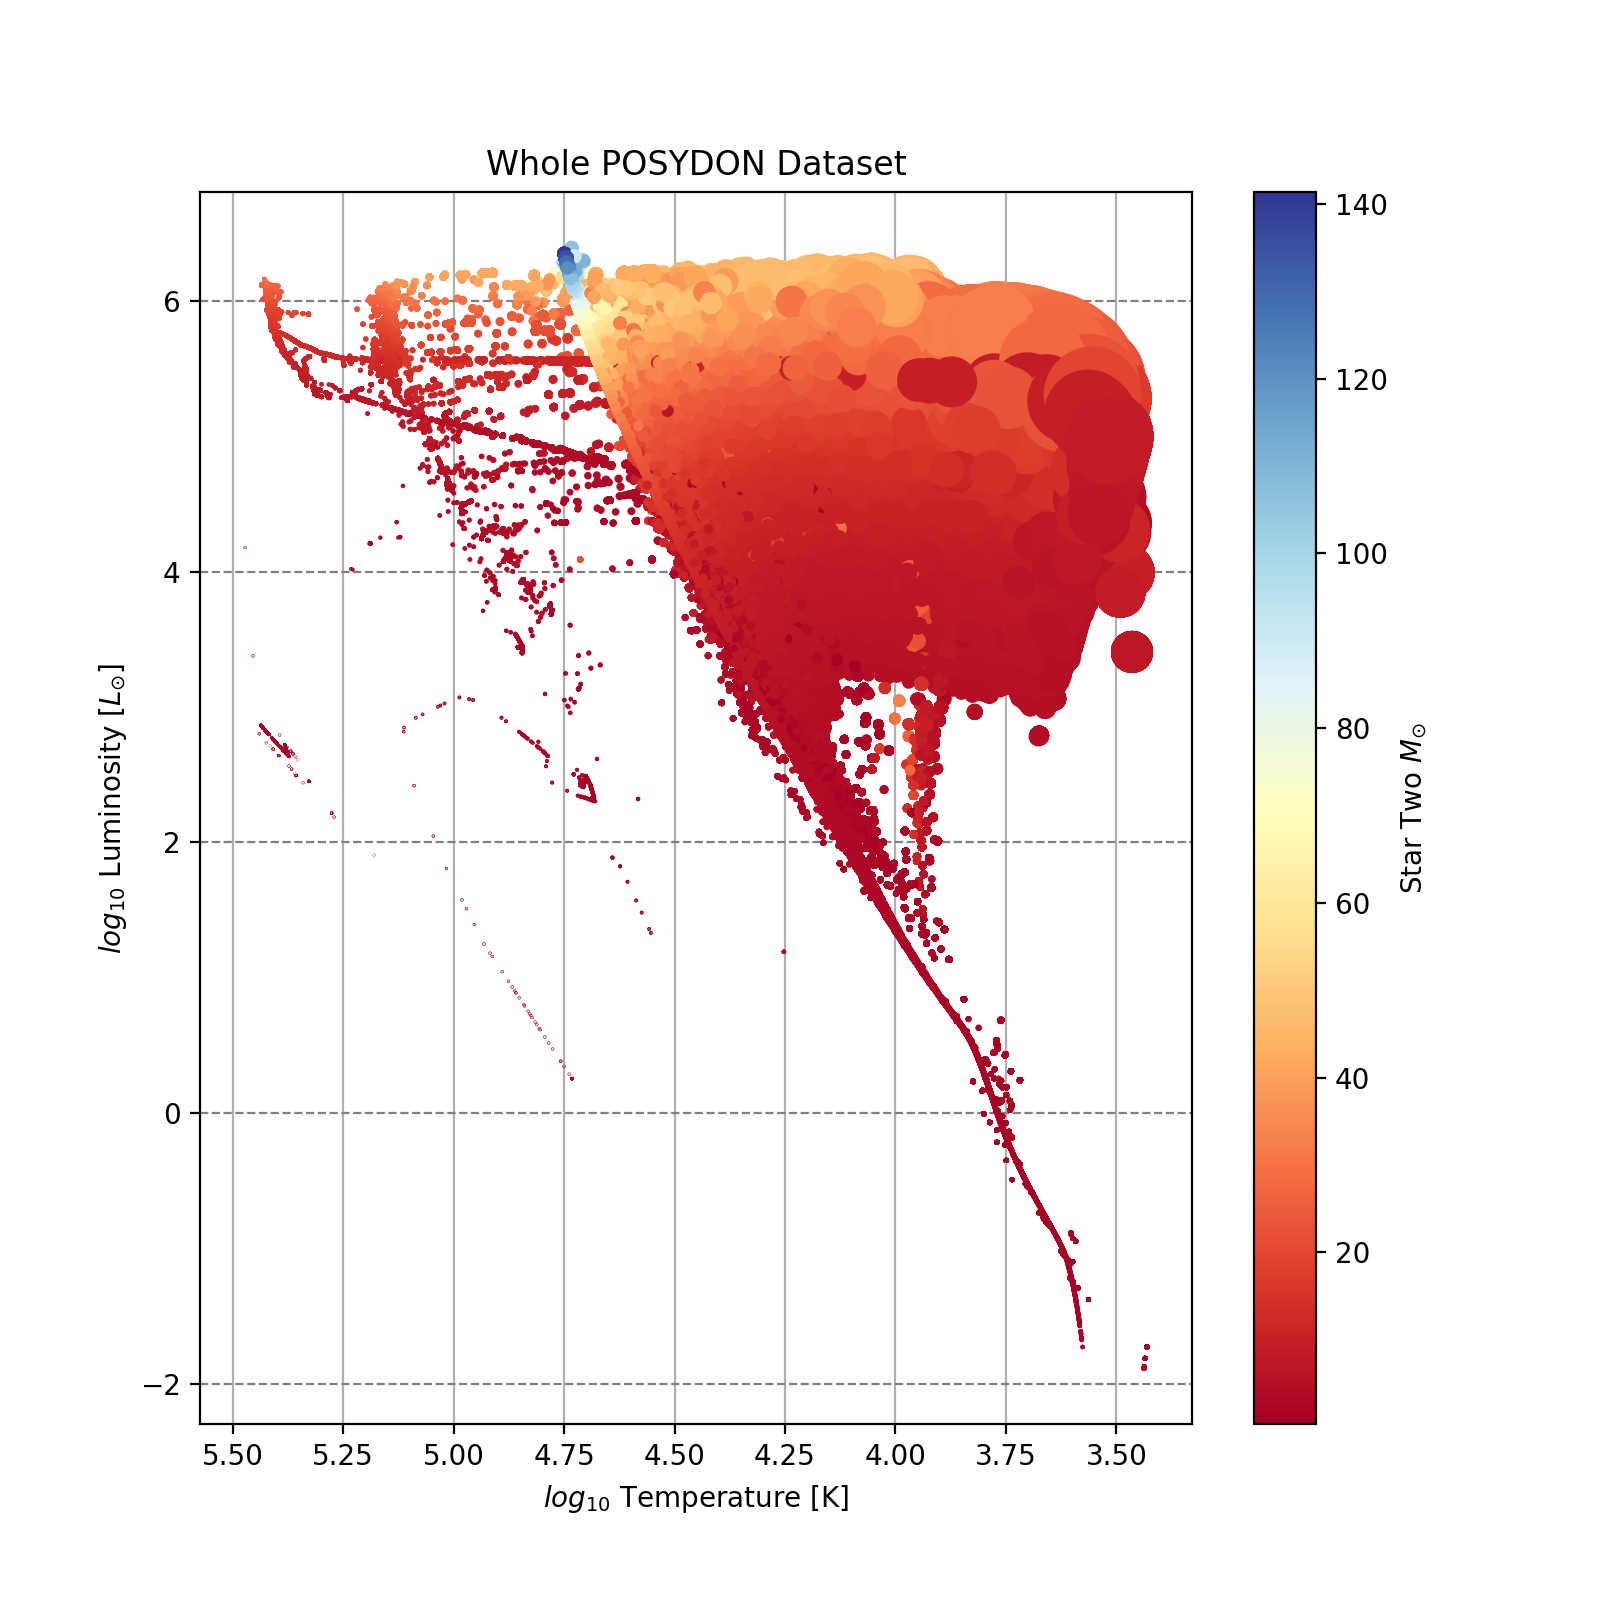
\includegraphics[scale = .5]{figs/GeneratedFigs/WholePOSYDONDatasetExample.png}
        \caption{Hertzsprung-Russell diagram of the donor star for the full POSYDON dataset meaning that this graph contains $\approx$6.1 million points. Note that the color of the plotted points correspond to the solar mass of the donor star. Additionally, the size of each plotted point is logarithmically related to the radius of the plotted star which it represents. This means that for each plotted point, one can evaluate four different variables, something which is rare in 2D graphs. I generated this figure utilizing Matplotlib and pandas.}
        \label{EntireDataSetHR}
    \end{figure}

    \begin{table}[H]
        \footnotesize
            \centering
            \begin{tabularx}{\textwidth}{||X|X|X|X|X|X|X|X||}
                \hline 
                \textbf{Binary ID} & 
                \textbf{System State} & 
                \textbf{Orbital Period (days)} & 
                \textbf{$\log_{10}$ Mass Transfer Rate} & 
                \textbf{Donor State} & 
                \textbf{Donor Mass} ($M_\odot$) & 
                \textbf{Accretor State} & 
                \textbf{Accretor Mass} ($M_\odot$) \\
                \hline \hline
                $1$ & Detached & $0.047520$ & $-99.00000$ & NS & $1.196033$ & Stripped He Core He burning & $\approx 1.002$ \\
                \hline
                \multicolumn{8}{||c||}{\textbf{\ldots}}\\
                \hline
                $1,000,000$ & Detached & $0.0429883$ & $\approx -80.8$ & NS & $1.196033$ & Stripped He Core He burning & $\approx 0.9957$ \\
                \hline
            \end{tabularx}
            \caption{Example of POSYDON data, heavily modified for readability.}
            \label{POSYDONDataExample}
        \end{table}
        


\section{Results}
    Through this paper I learned a massive amount about the processes of mass transfer in binary stars now feel that I could speak fluently about the topic. I learned a lot about the physics and math involved in the process and how crucial of a part it plays in the evolution of binary systems. Additionally, I furthered my data analysis skills in Python, learning how to greatly refine said process. Furthermore, I learned how to use \LaTeX~for academic writing and how to streamline a workflow consisting of Python, Git, GitHub, and VS Code.

    I found a lot of the key factors in mass transfer and how it affected various types of binary stars, with Full-blown RLO being the most key factor in mass transfer in low-mass x-ray binaries, leading to large amounts of x-ray emission. This process had drastic effects on both the donor and accretor star. Full-blown RLO is when mass itself is directly transferred between the two stars.

    Counterintuitively, I found that a large quantity of detached systems (systems where neither star has filled their Roche Lobe) will experience mass transfer in some form. This mass transfer is in the form of wind accretion or atmospheric Roche Lobe Overflow.

    Furthermore, I found that mass can will be transferred between stars in contact binaries, with a majority of contact binaries not actually being stable, but instead in a phase of their life called common envelope.

    Lastly, I found that in systems with low mass donor stars mass transfer will occur directly through the Lagrange point $L_1$. This process of mass transfer will lead to a considerable increase in x-ray emissions which can be measured and evaluated from earth.
    
    \subsection{Original Results}
        I found that V404 Cyngi properties did not fall onto a known location on an HR Diagram, something which is incredibly unusual (fig. \ref{V404Cygni}). This suggests that either the simulated data generated using POSYDON has an error, or that observed data is incorrect. Of the two it is much more likely that there is a fault with POSYDON (or even MESA itself) when it comes to simulating LMXBs. This could pose a larger issue, as a lot of papers utilize POSYDON and/or MESA to come to their conclusions. 
        
        \begin{figure}[H]
            \centering
            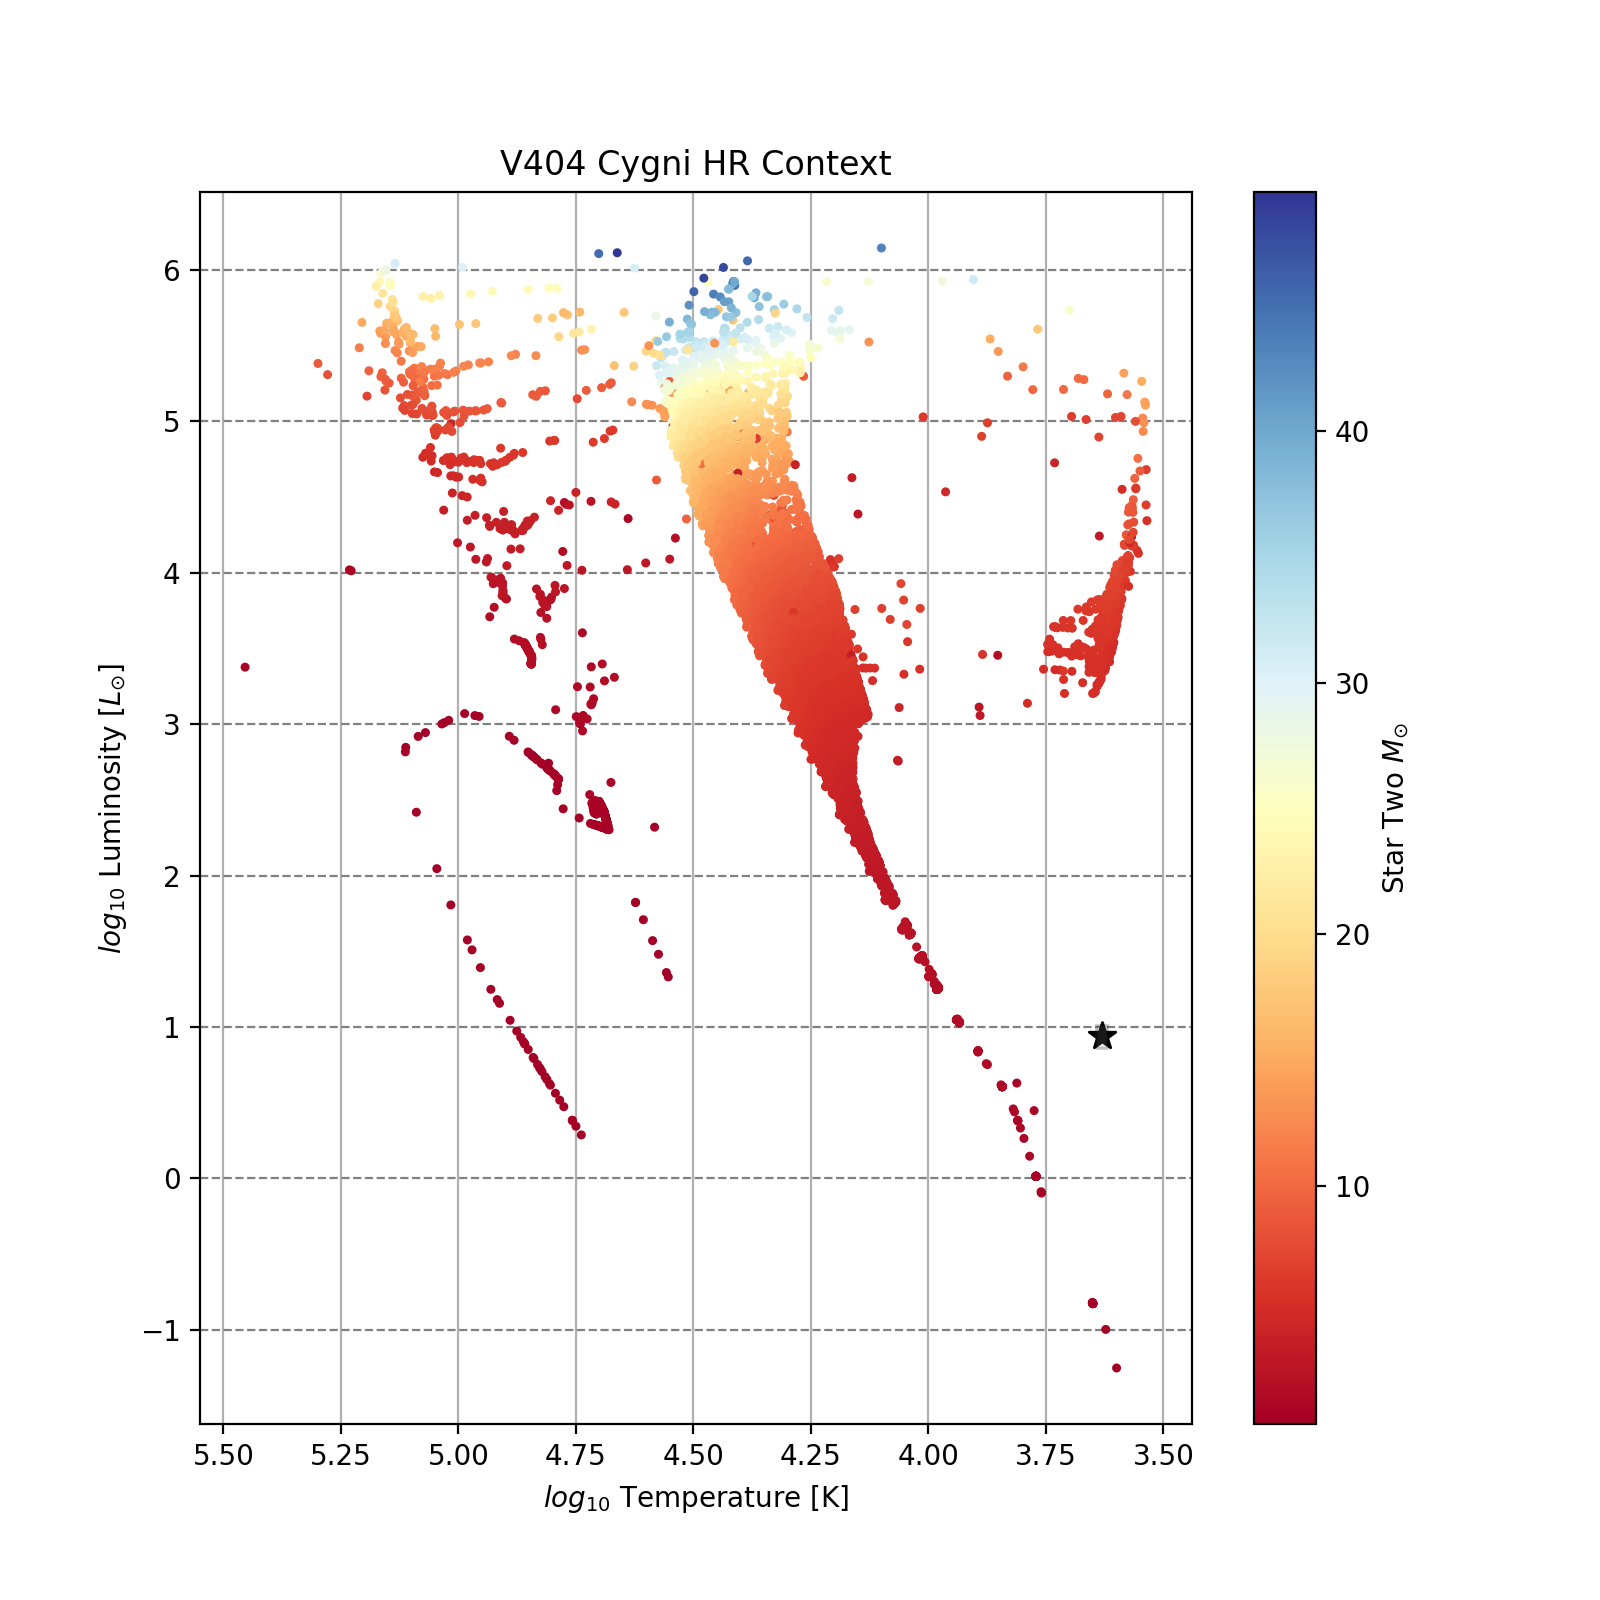
\includegraphics[width = .6\textwidth]{figs/GeneratedFigs/V404_Cygni/V404XBsPopulationHRComp.png}
            \caption{Hertzsprung-Russell diagram comparing V404 Cygni with simulated stars of the same type. The properties of V404 Cygni are located at the black star. Note that it falls in a unique location compared to stars of the same type. Graphing using Matplotlib and Pandas.}
            \label{V404Cygni}
        \end{figure}

        Additionally, I found a trend between the $\log_{10}$ luminosity $L_{\odot}$ and $\log_{10}$ temperature $K$ in contact binaries, with contact binaries falling on a specific evolutionary track (see fig. \ref{ContactBinaryTrack}). This result should be taken with a grain of salt however, as current simulated models of contact binaries are known to simulate systems with higher temperature and luminosity then is observed, something I corroborated with my data.

        \begin{figure}[H]
            \centering
            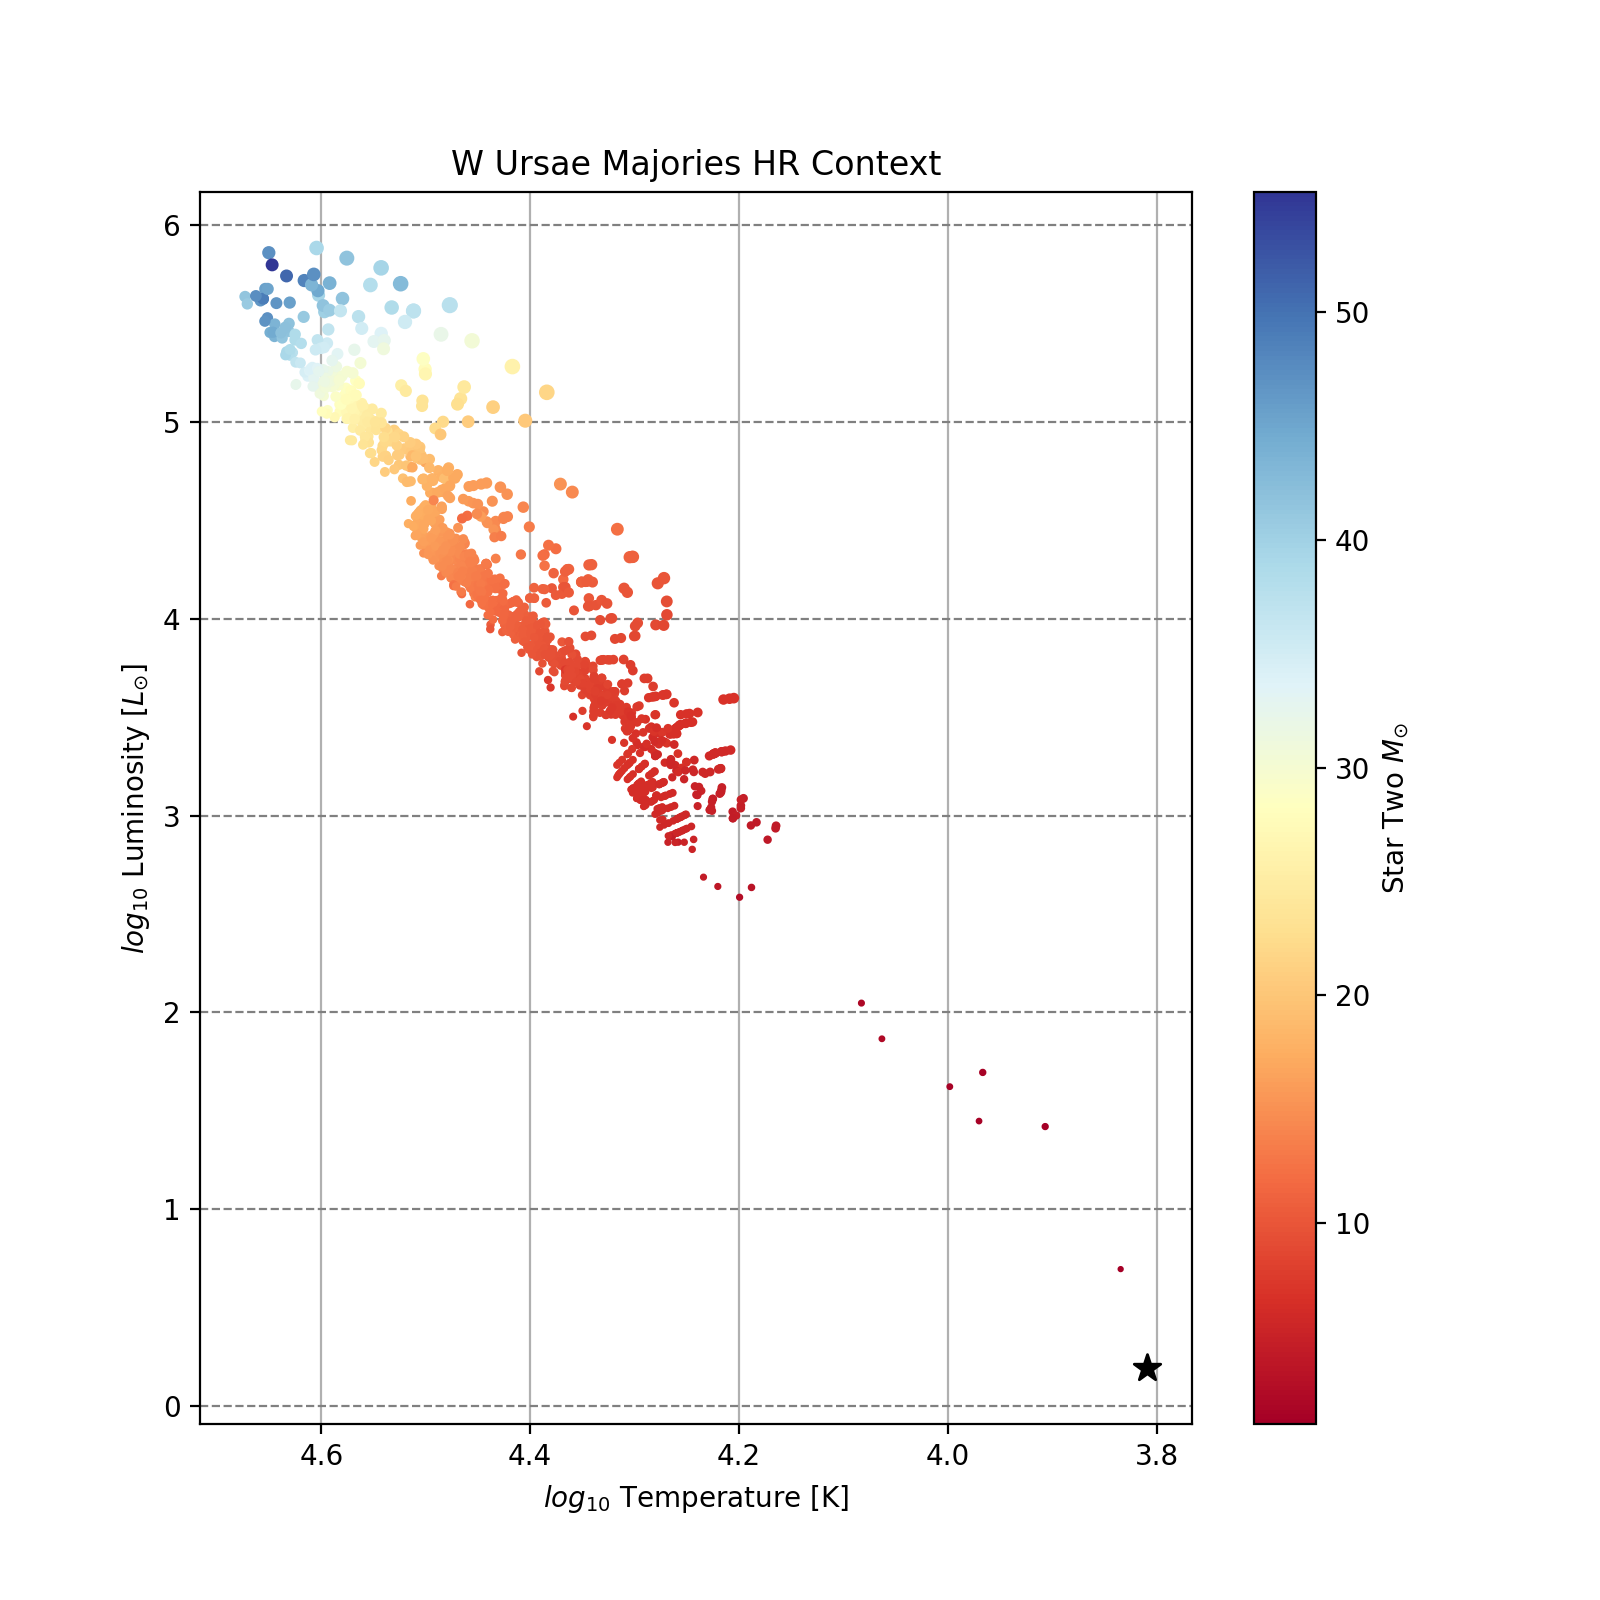
\includegraphics[width = .6\textwidth]{figs/GeneratedFigs/W_UMa/WUMaHRDiagram.png}
            \caption{Hertzsprung-Russell diagram comparing W Ursae Majoris with simulated stars of the same type. The properties of W UMa are located at the black star. Graphing using Matplotlib and Pandas.}
            \label{ContactBinaryTrack}
        \end{figure}
        

        I found that Vela X-1 is one of the more extreme examples within its population type, having a much greater luminosity and temperature then the greater population.

        \pagebreak
\begin{center}
    \textbf{These are all the figures I graphed and included in my paper.} 
    \begin{tabular}{cccc}
        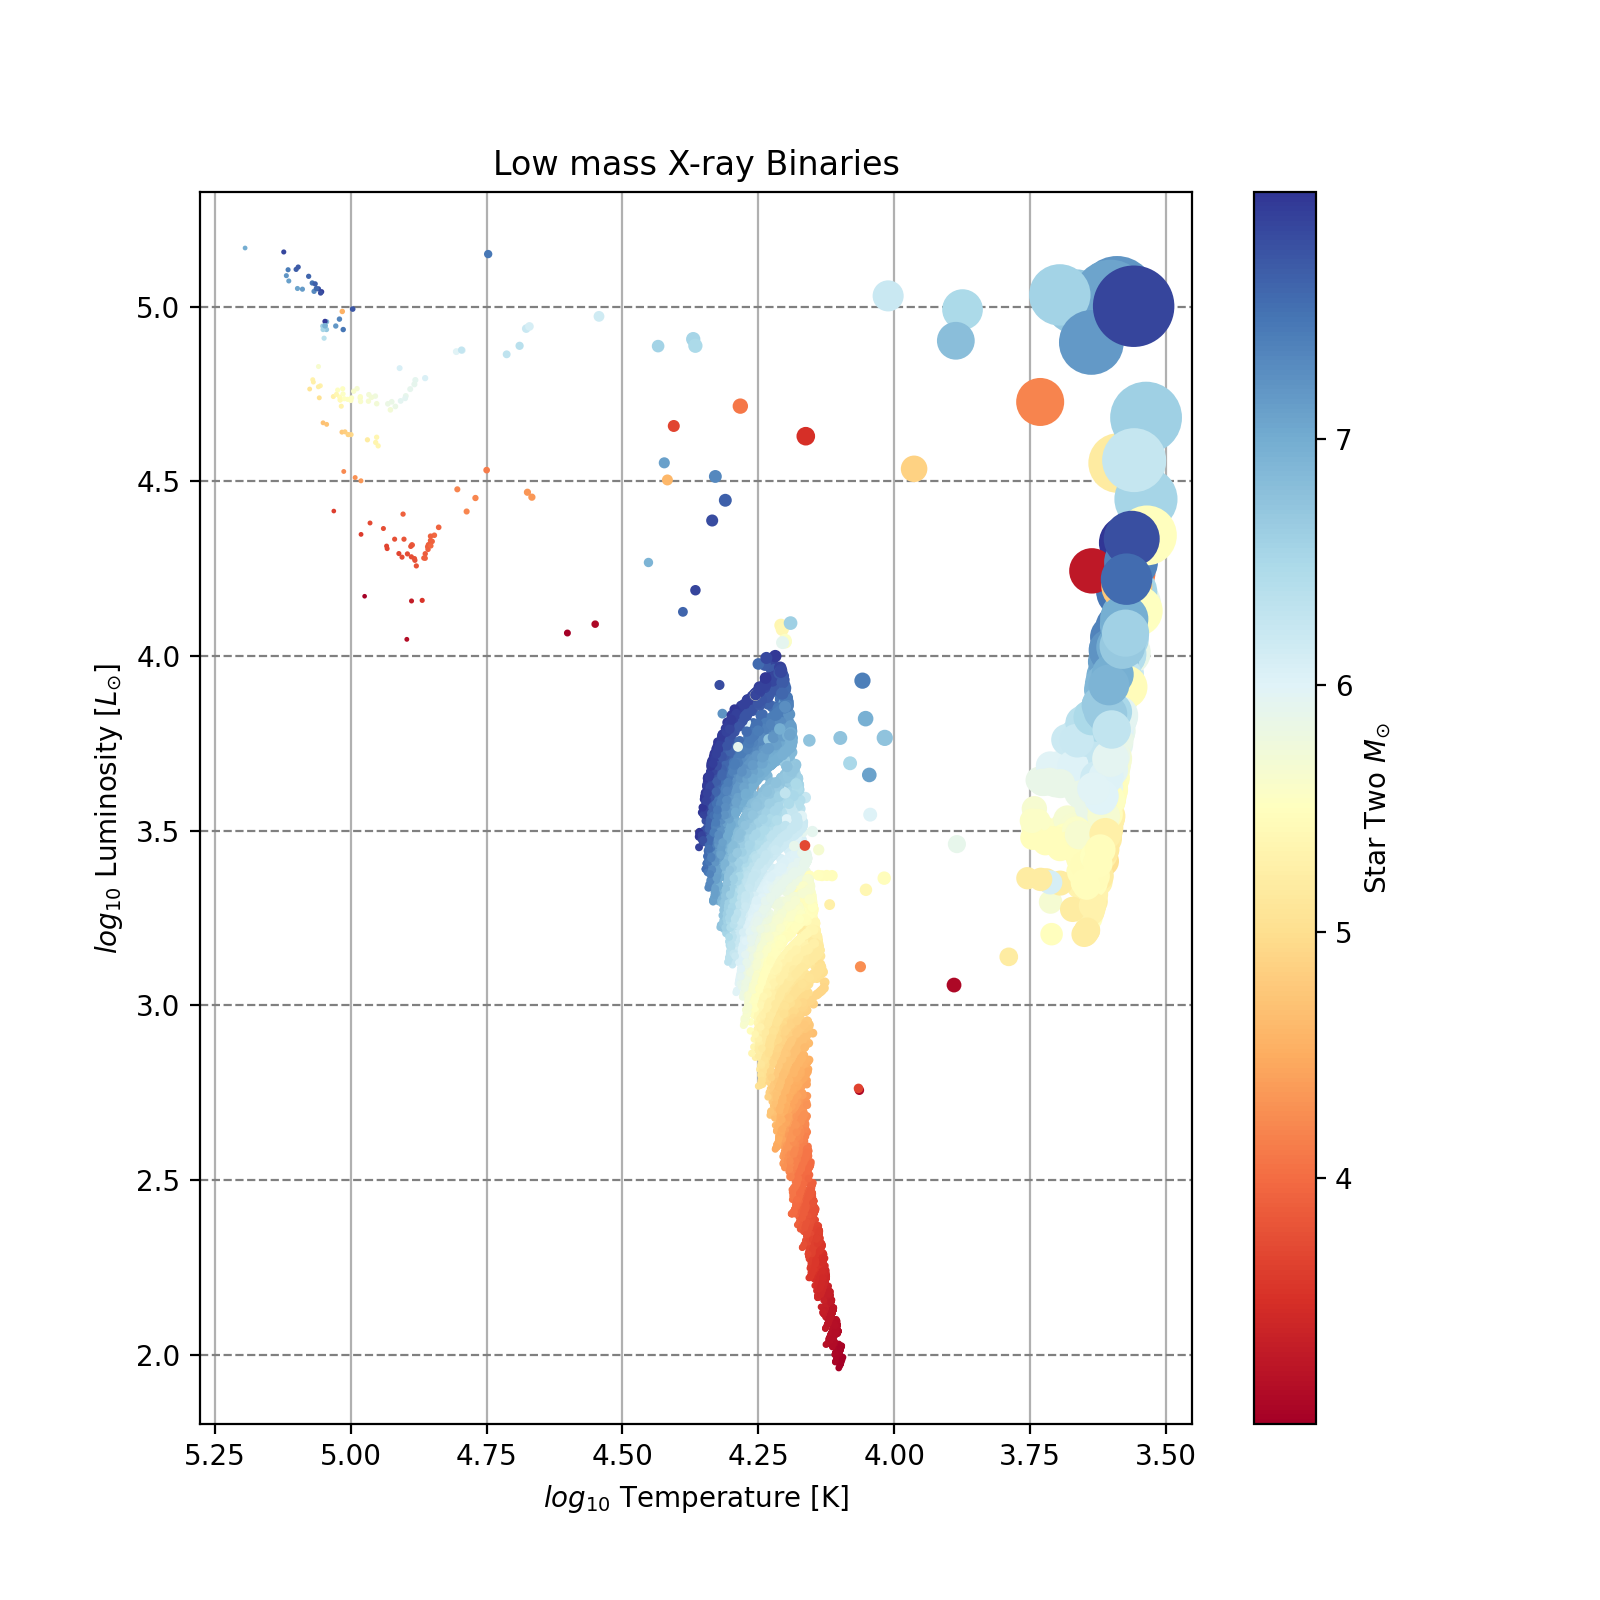
\includegraphics[width=0.22\textwidth]{figs/GeneratedFigs/V404_Cygni/LMXBsHRDiagram.png} &
        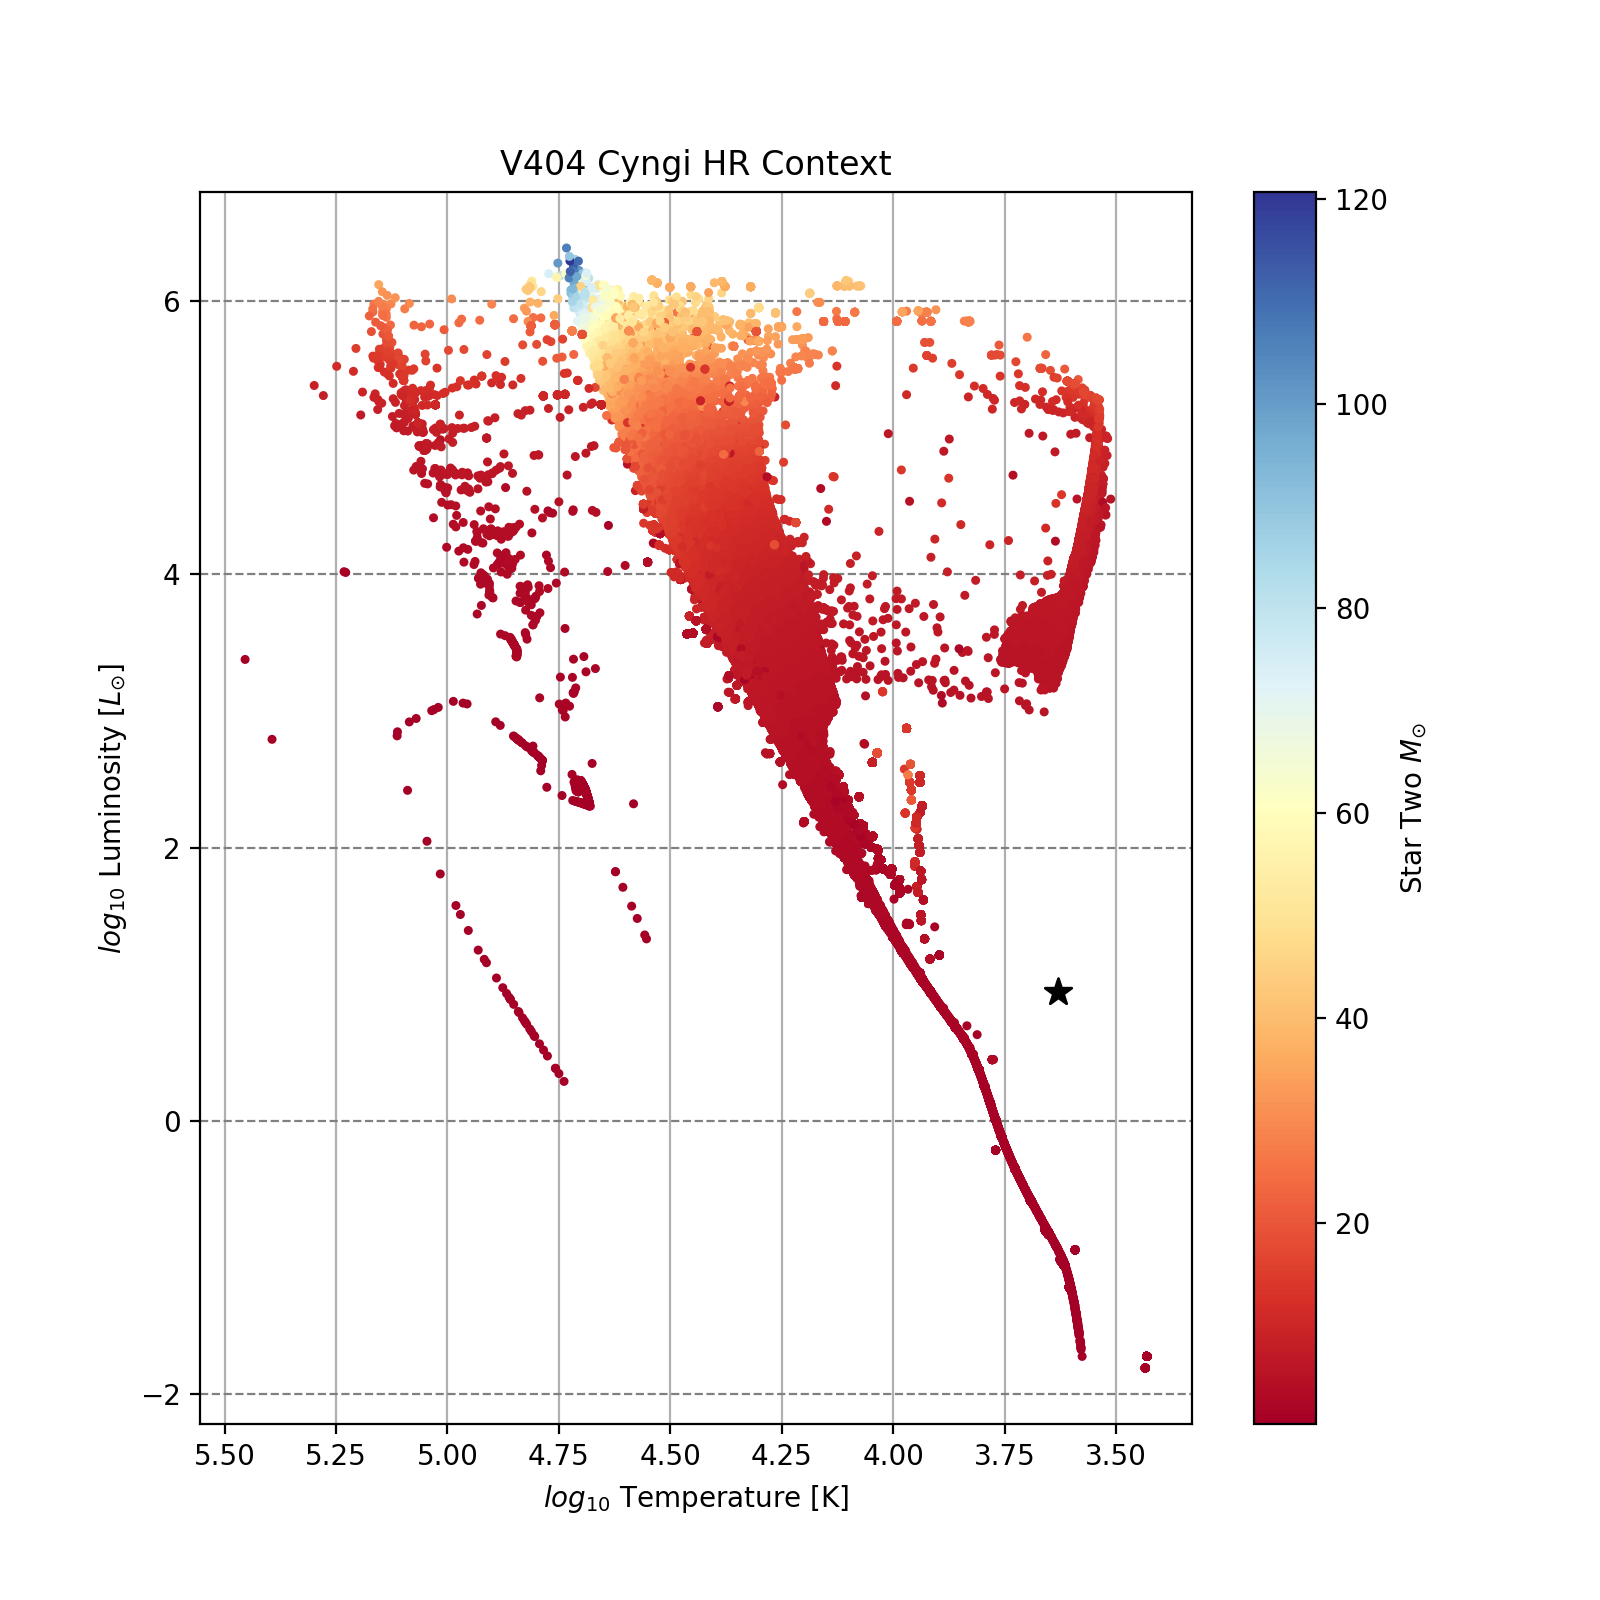
\includegraphics[width=0.22\textwidth]{figs/GeneratedFigs/V404_Cygni/V404EndStateDatasetPopulationHRComp.png} &
        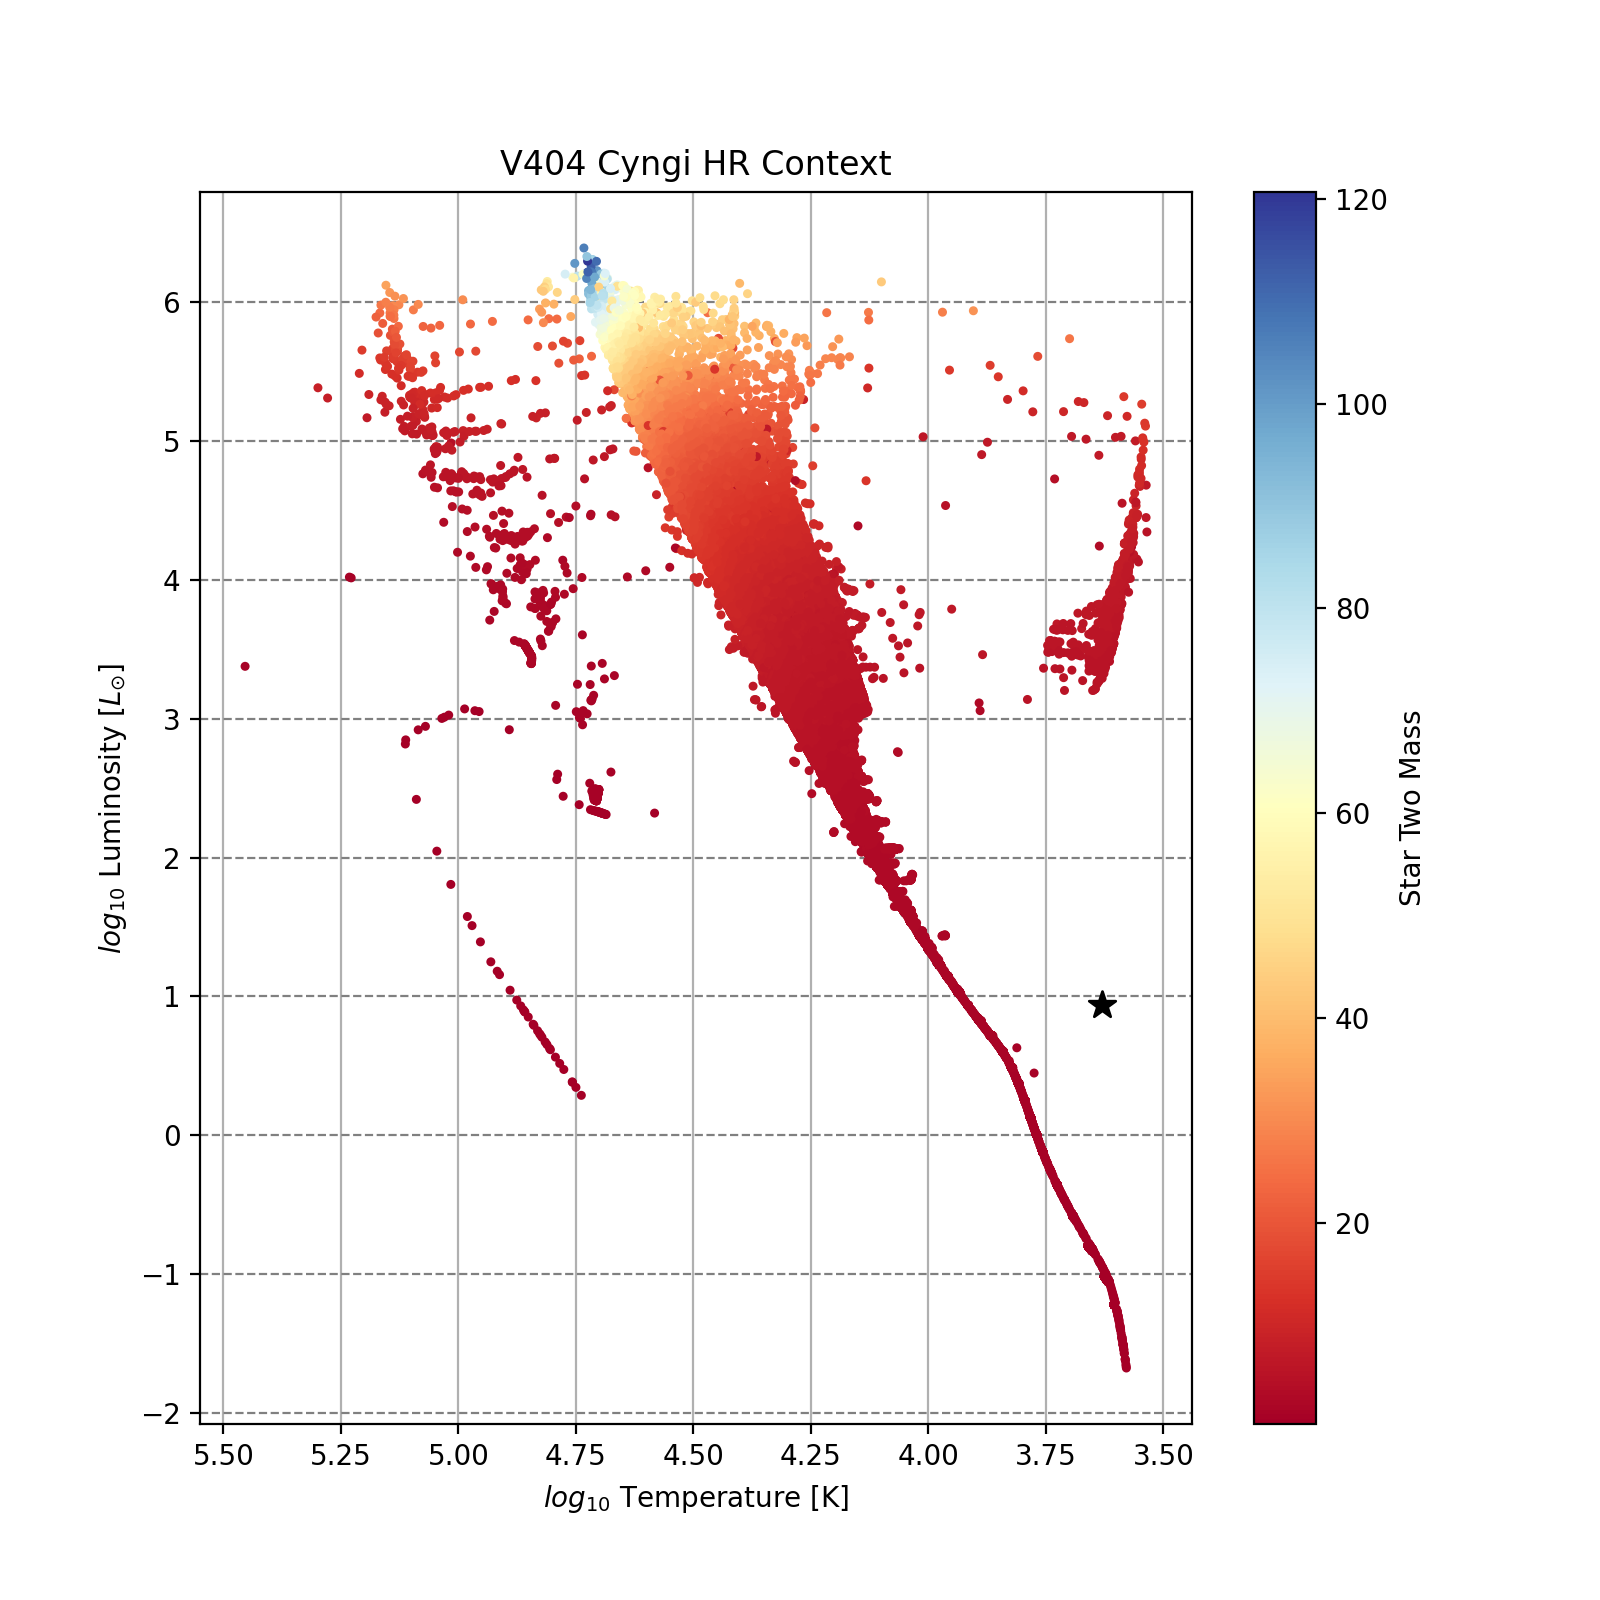
\includegraphics[width=0.22\textwidth]{figs/GeneratedFigs/V404_Cygni/V404LMXBPopulationHRComp.png} &
        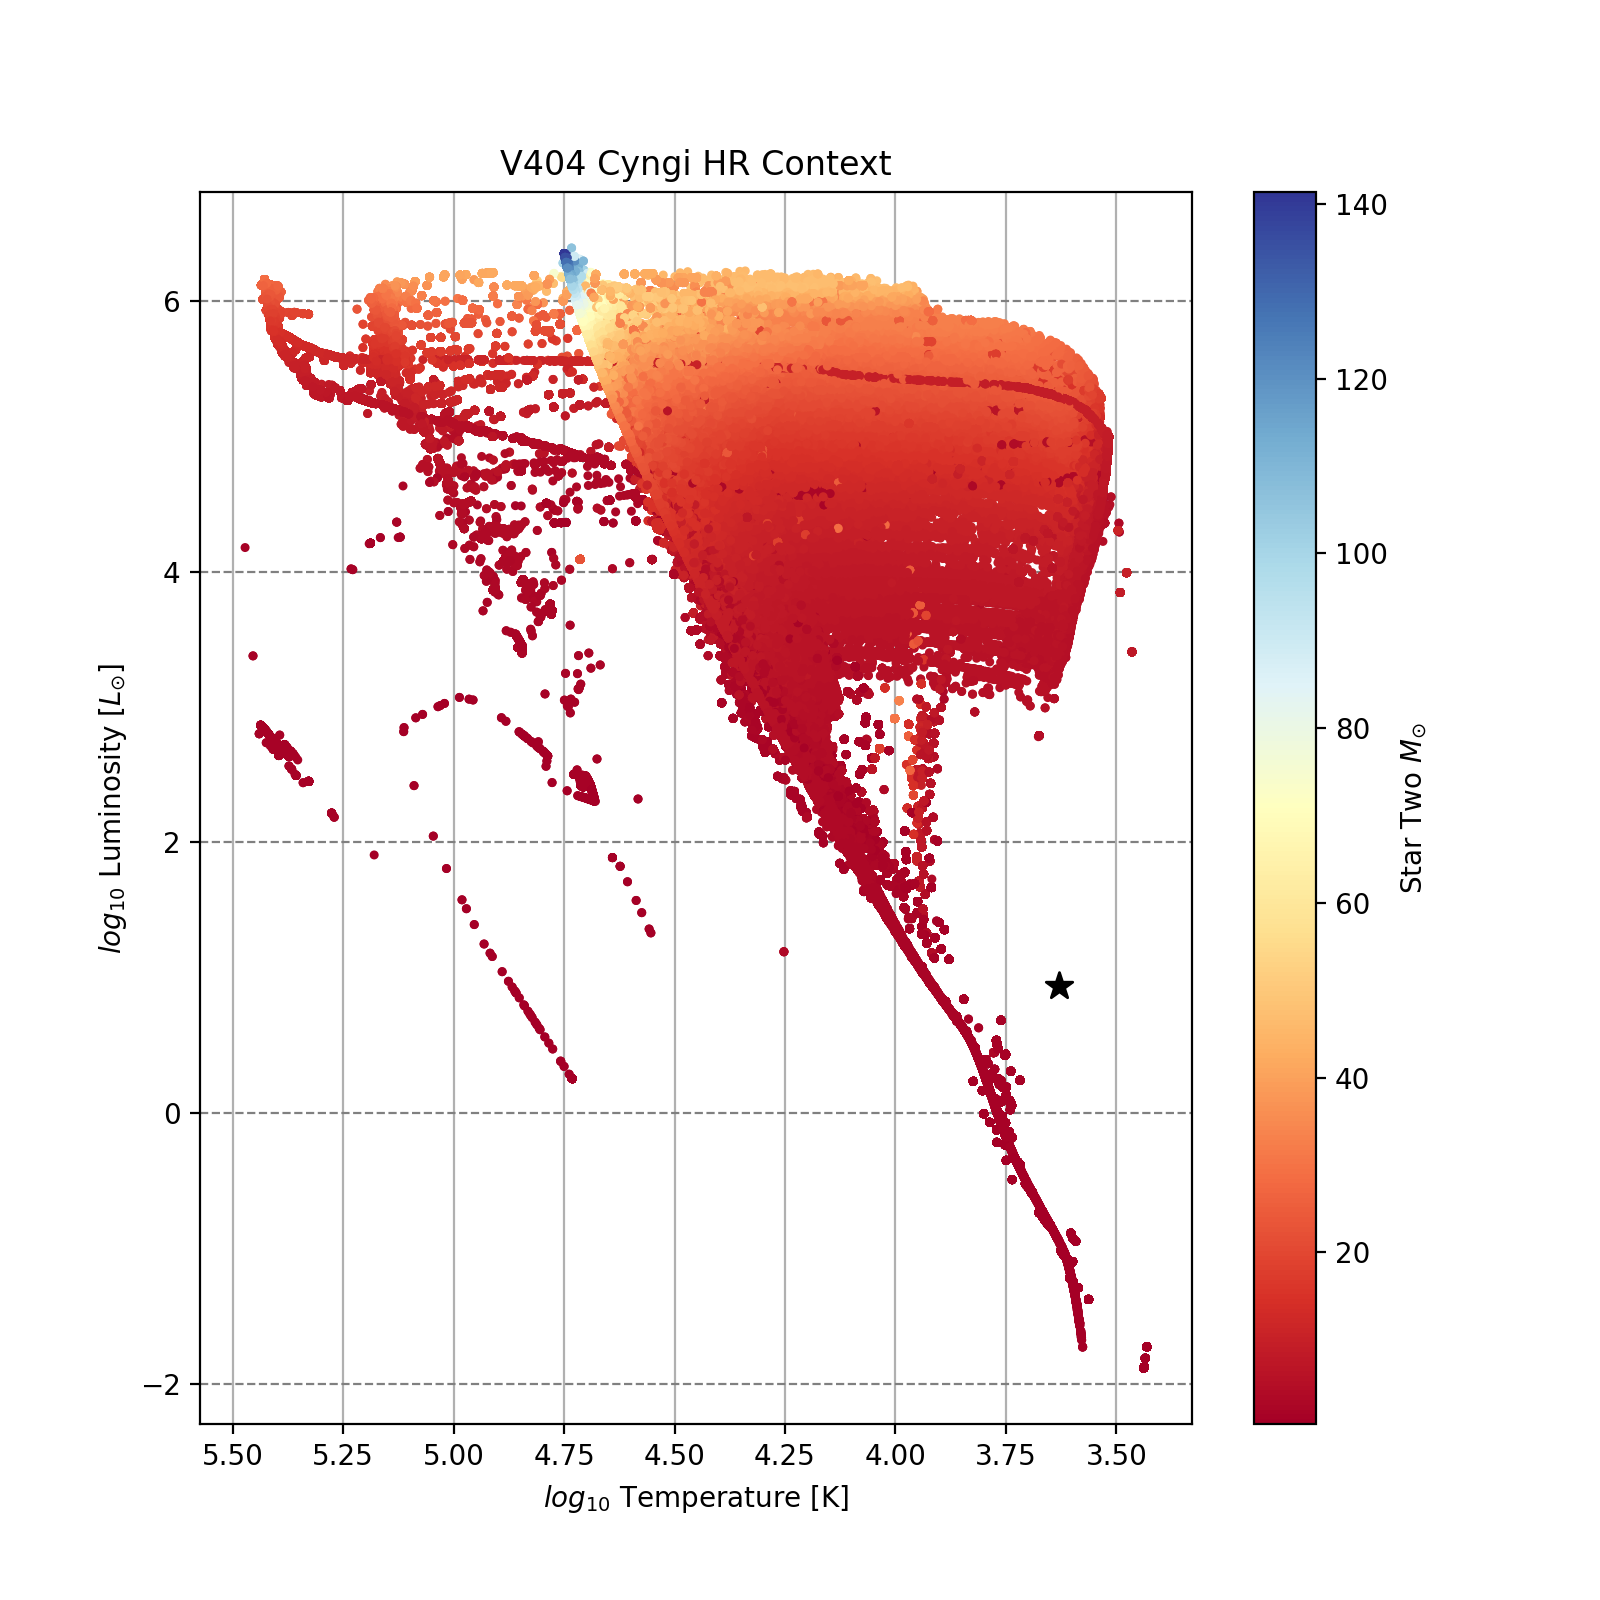
\includegraphics[width=0.22\textwidth]{figs/GeneratedFigs/V404_Cygni/V404EntireDatasetPopulationHRComp.png} \\
        
        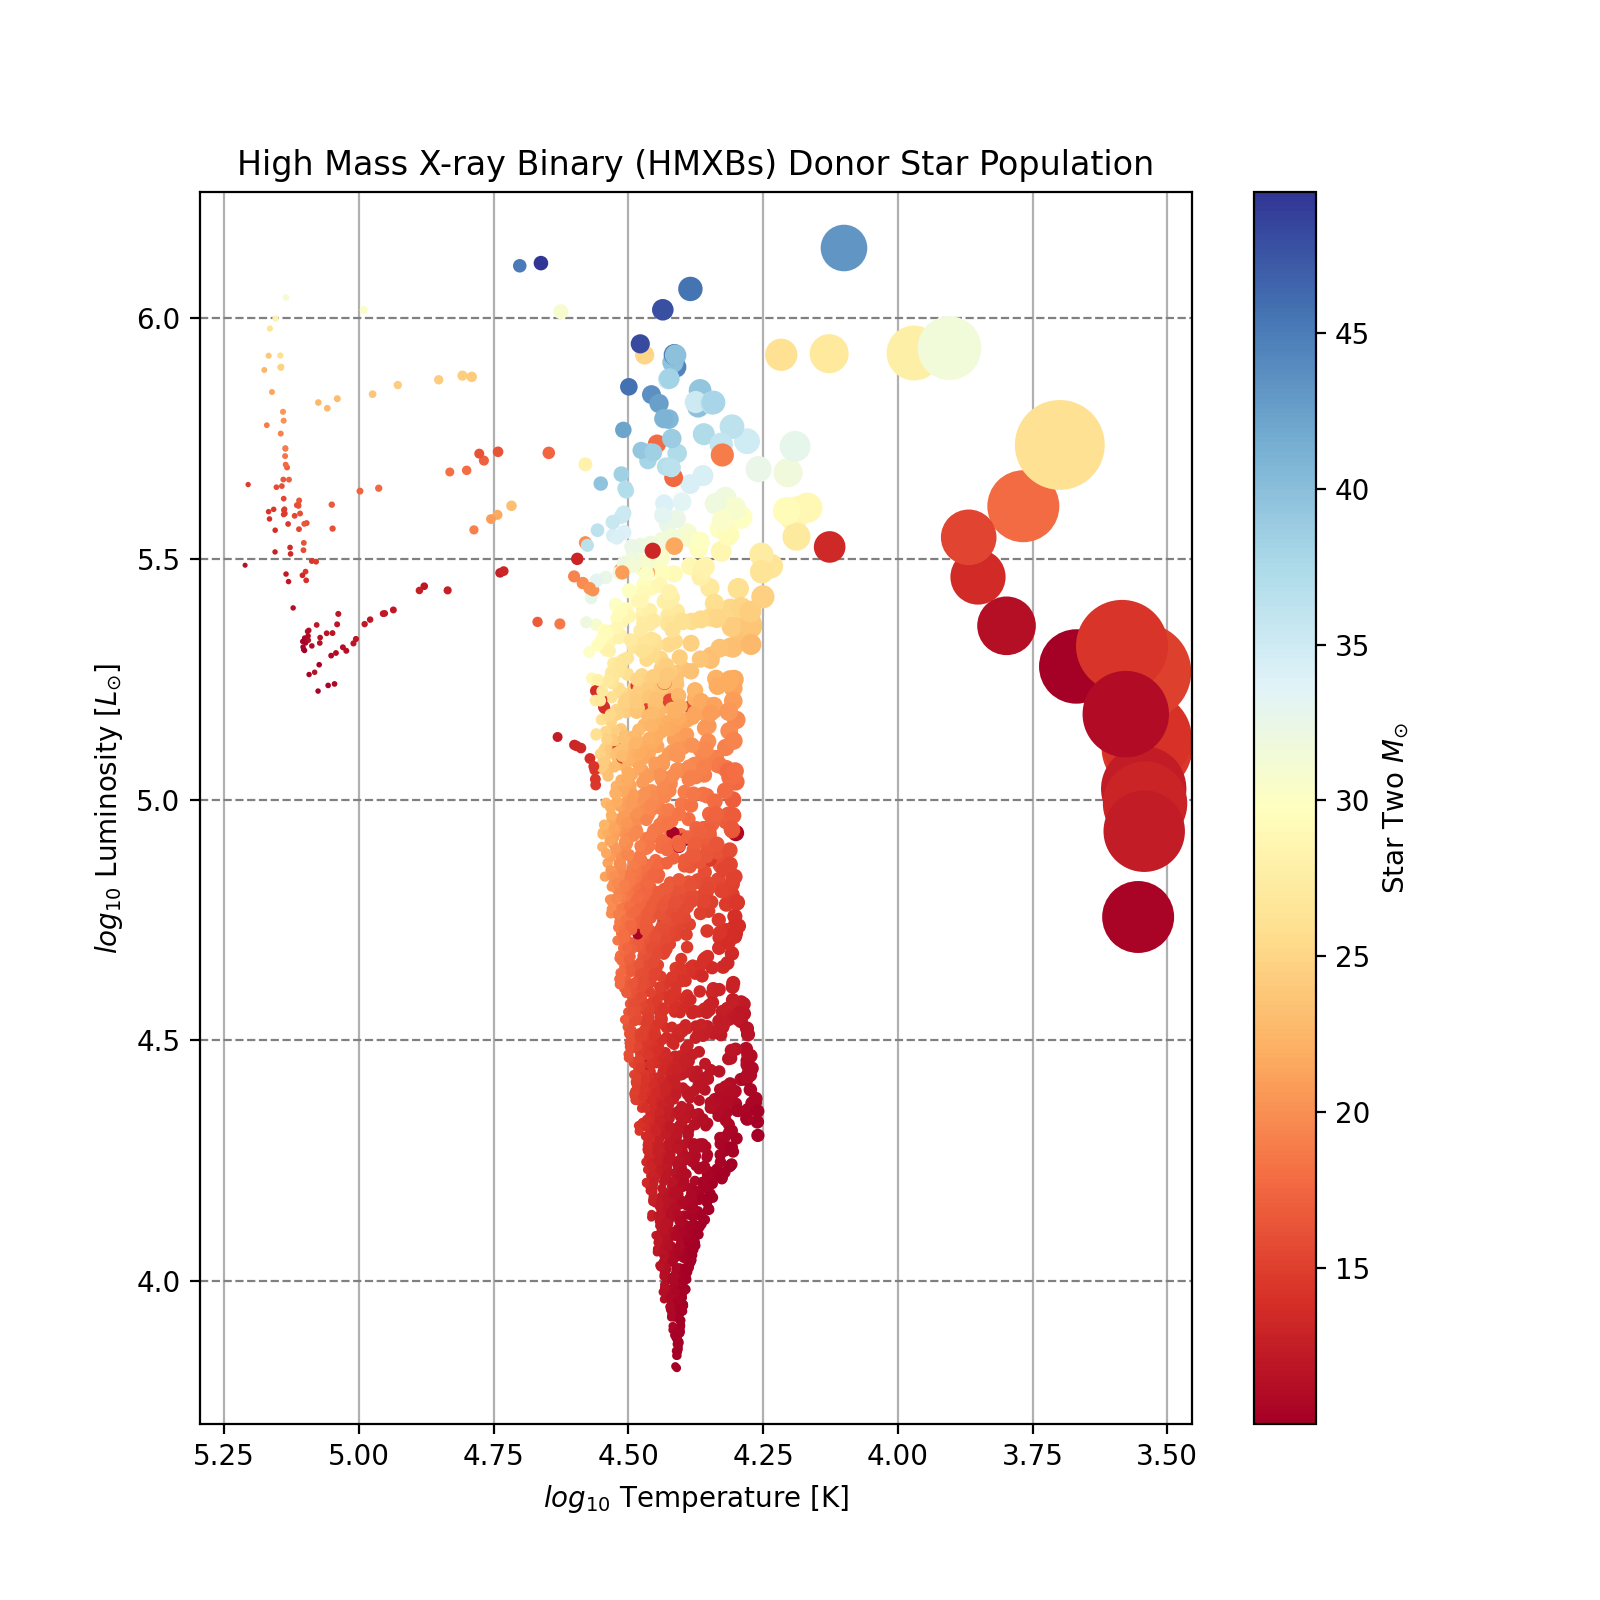
\includegraphics[width=0.22\textwidth]{figs/GeneratedFigs/VelaX-1/HMXBHRPopulation.png} &
        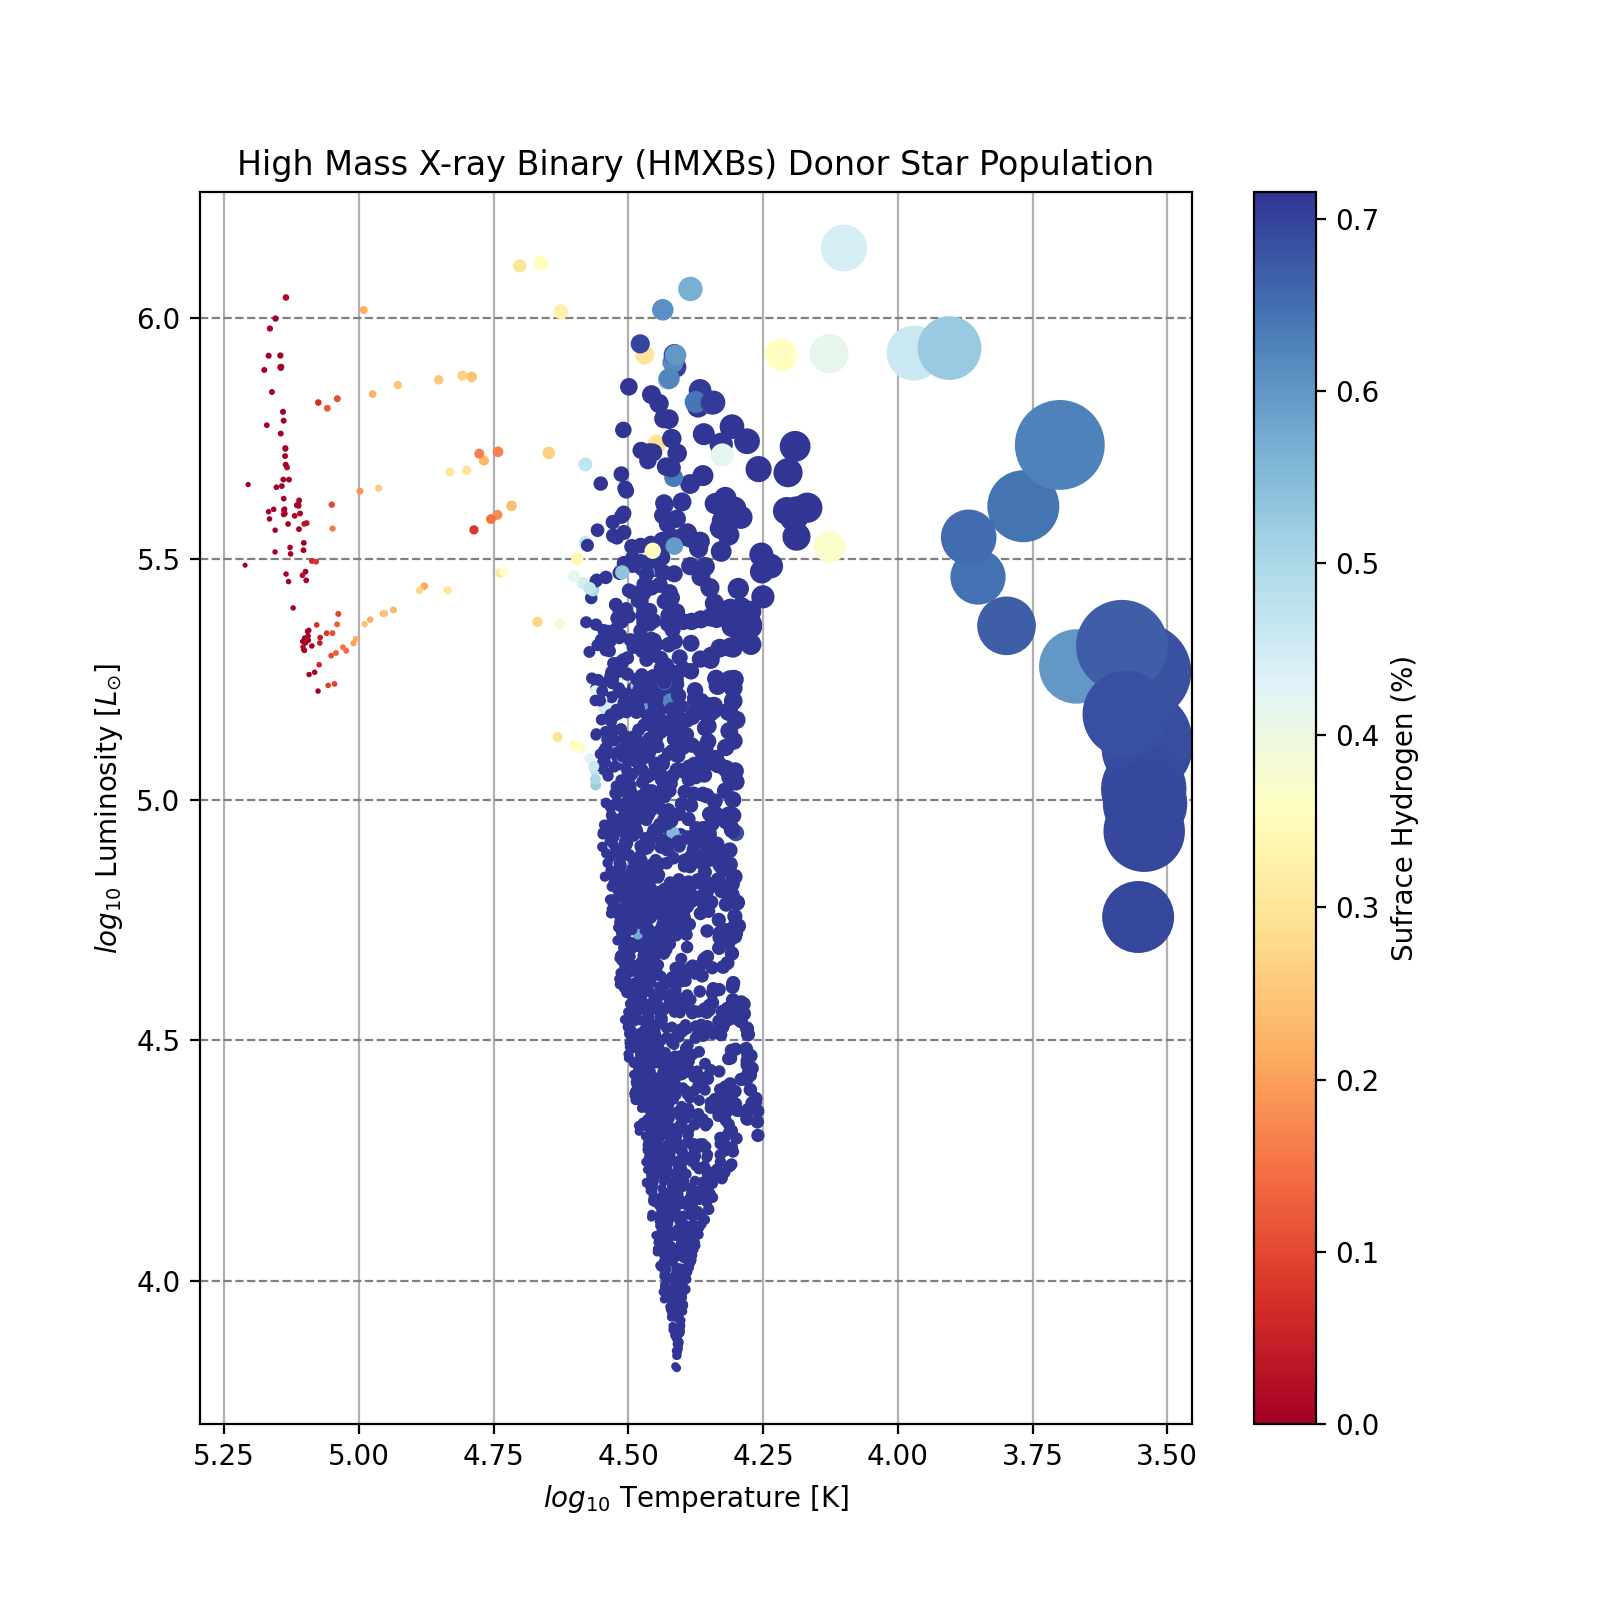
\includegraphics[width=0.22\textwidth]{figs/GeneratedFigs/VelaX-1/HMXBsSurfaceCompHRDiagram.png} &
        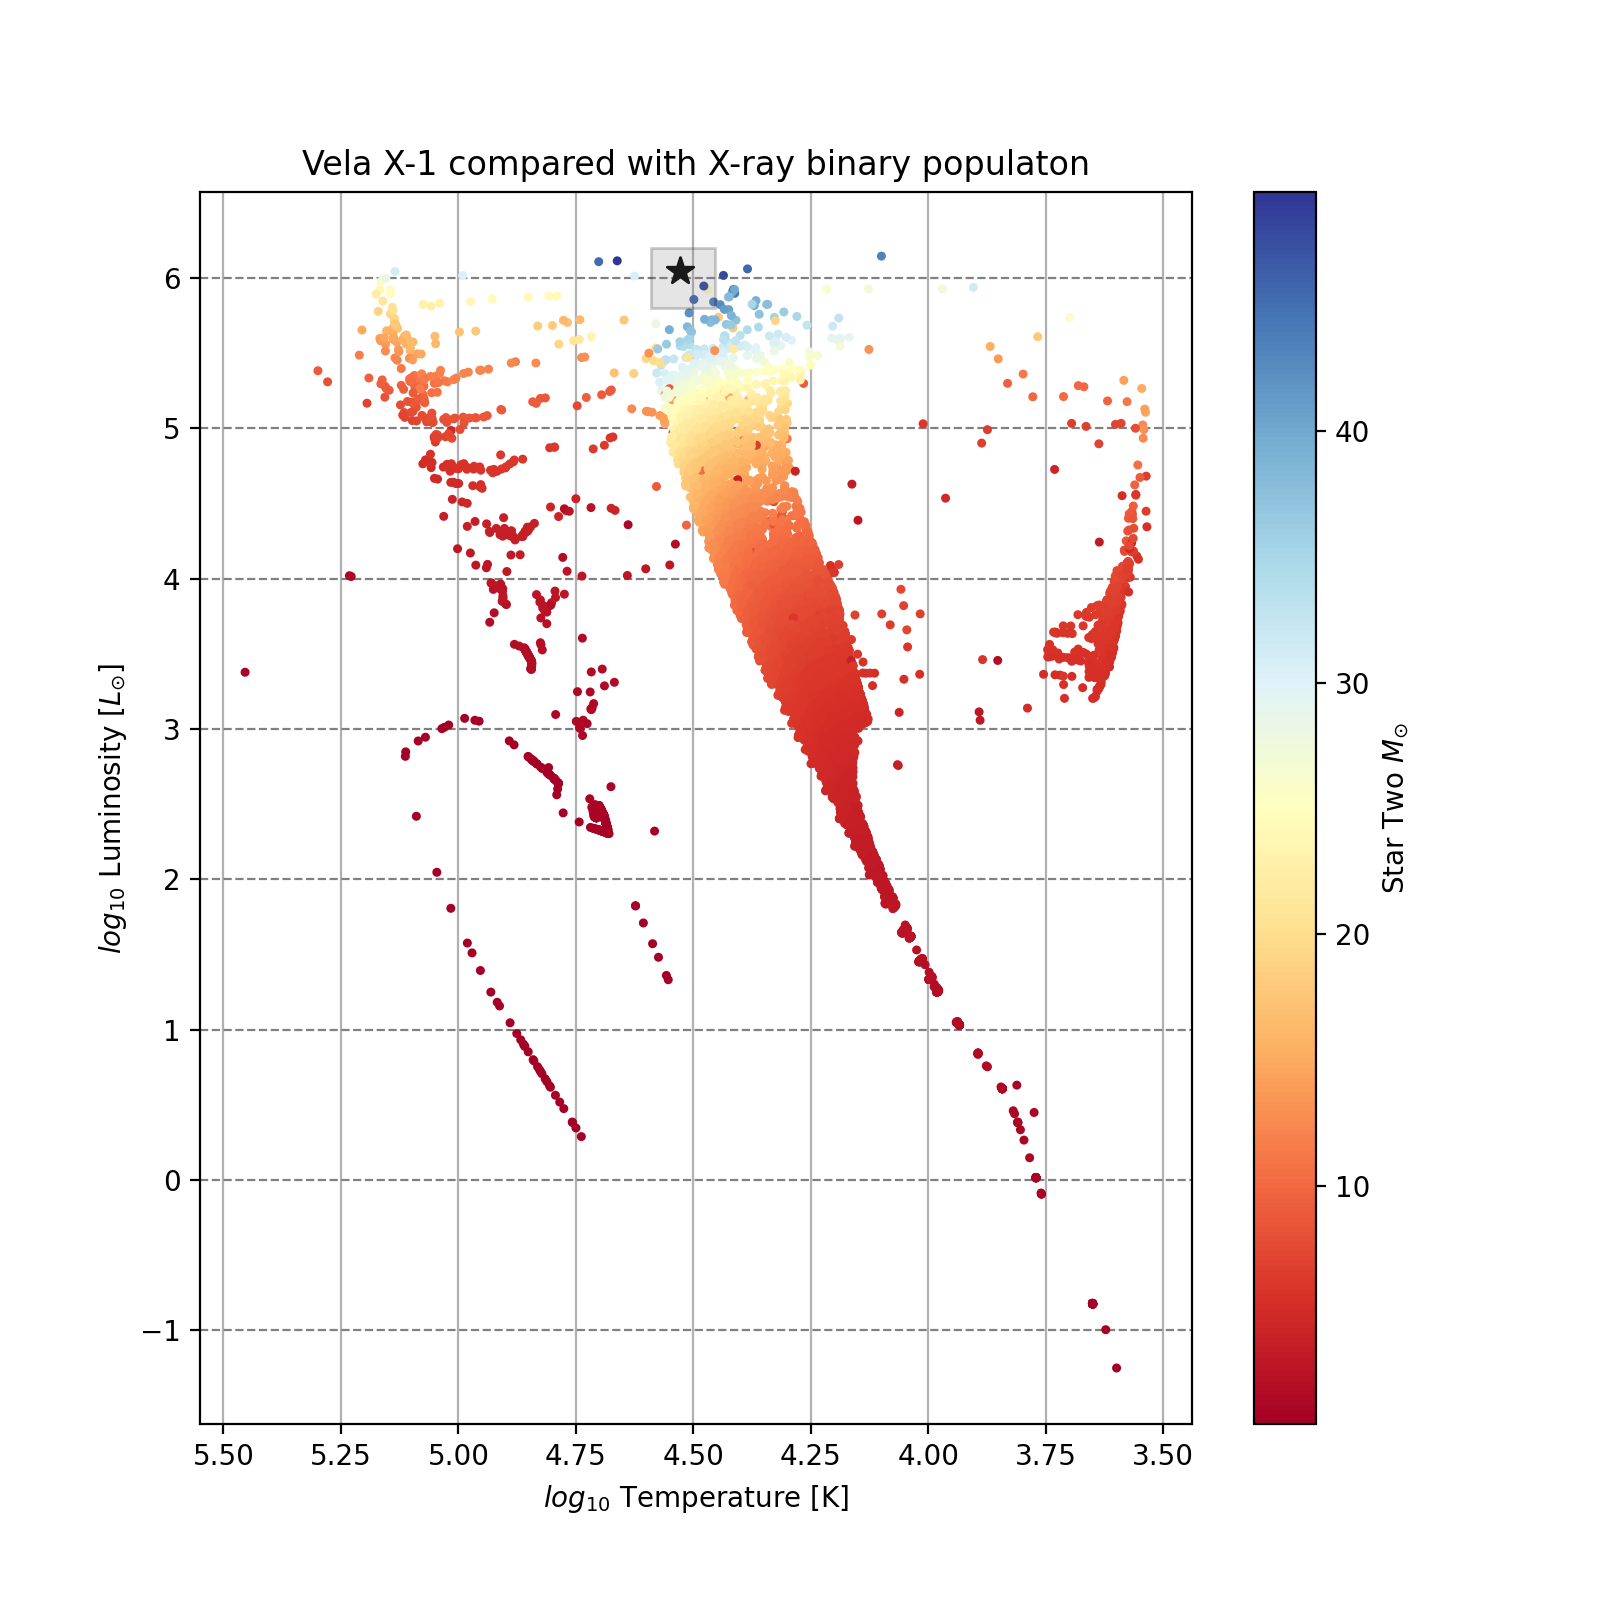
\includegraphics[width=0.22\textwidth]{figs/GeneratedFigs/VelaX-1/VelaX1XrBPopulationHRComp.png} &
        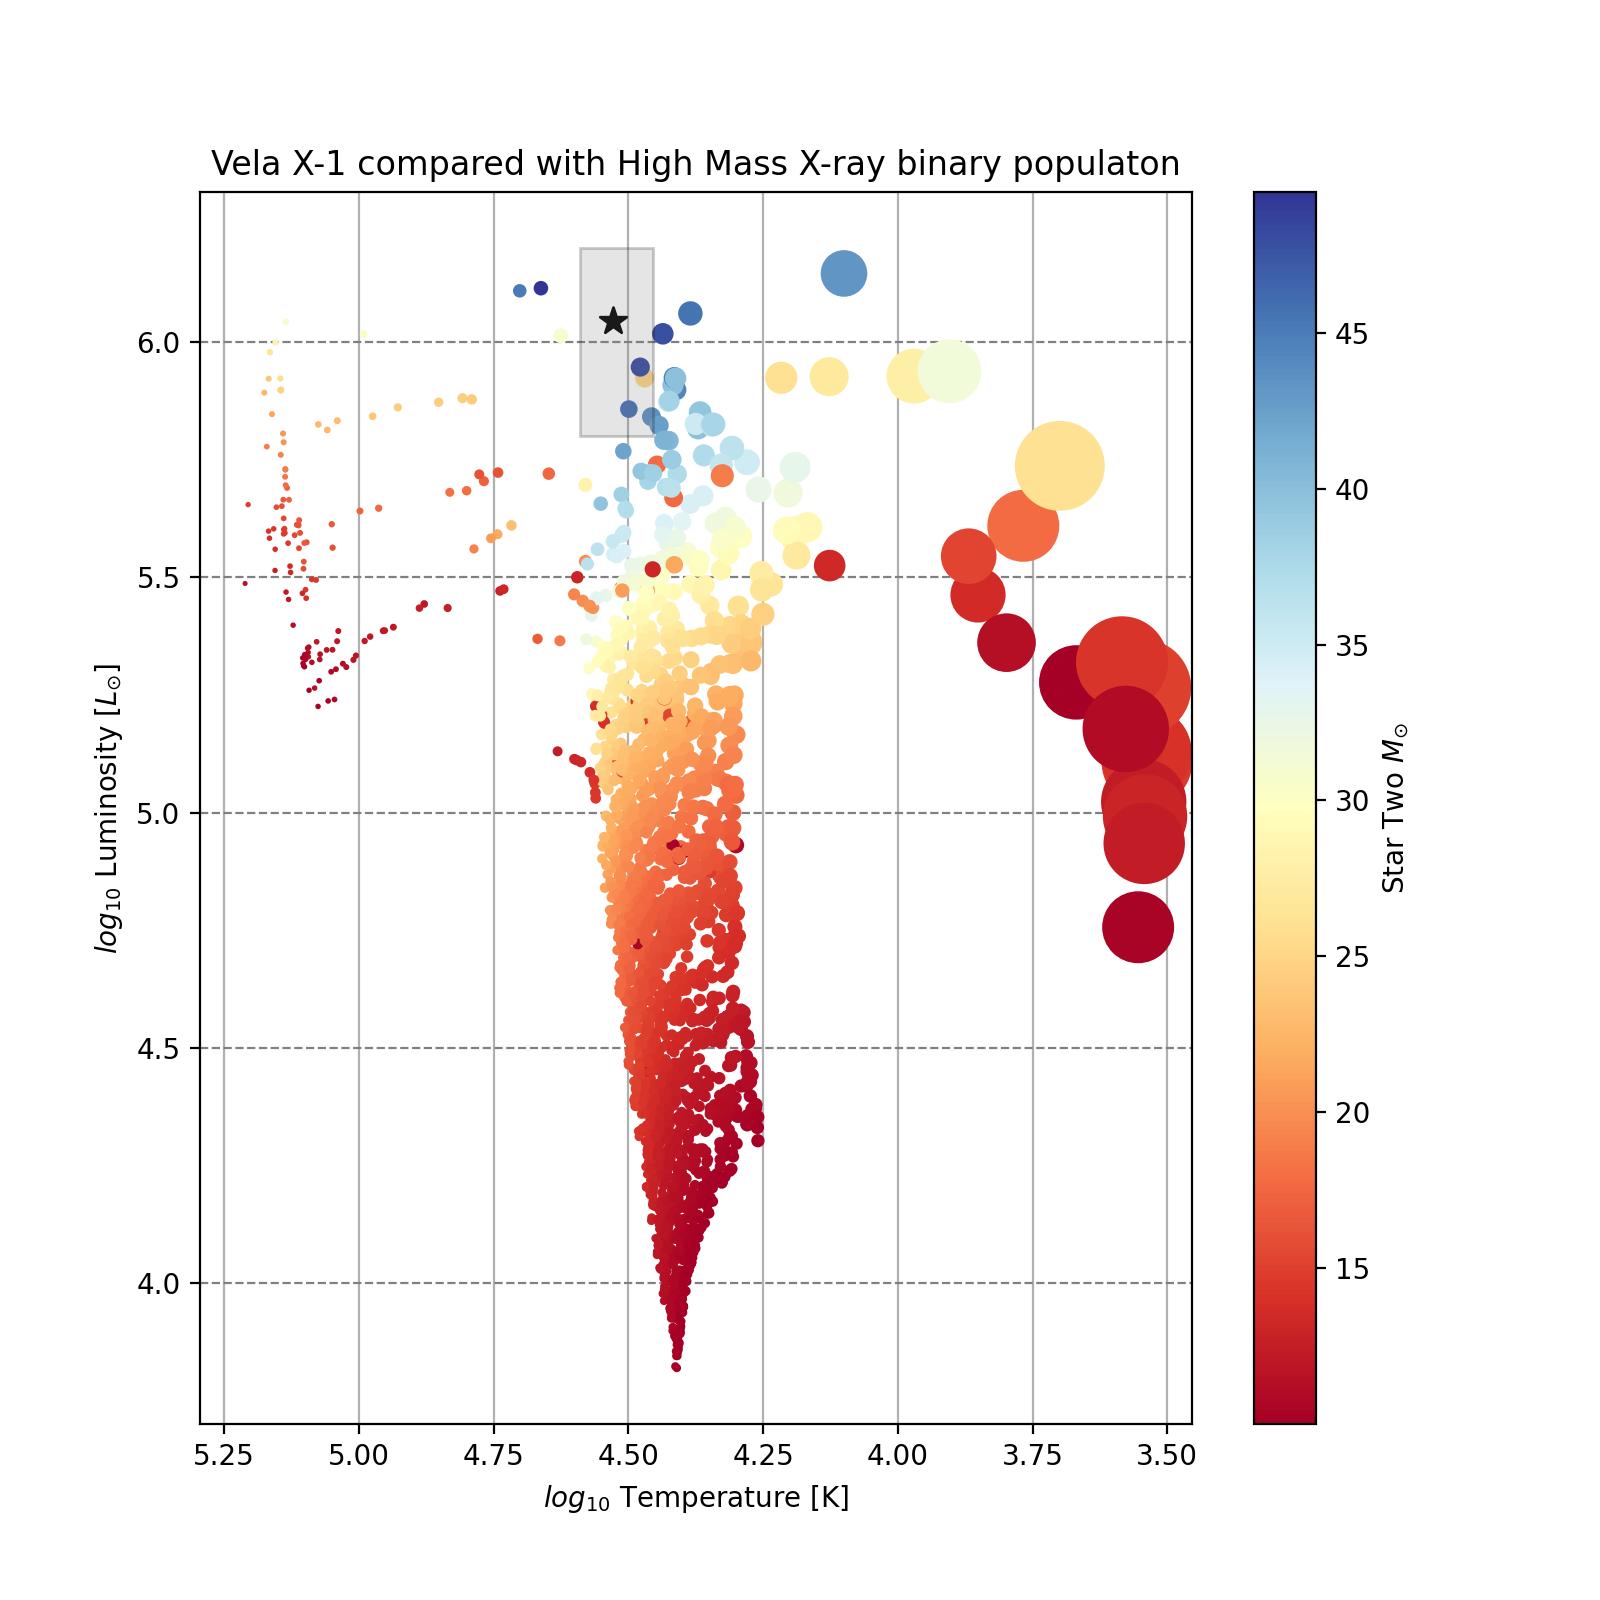
\includegraphics[width=0.22\textwidth]{figs/GeneratedFigs/VelaX-1/VelaX1HMXBPopulationHRComp.png} \\
        
        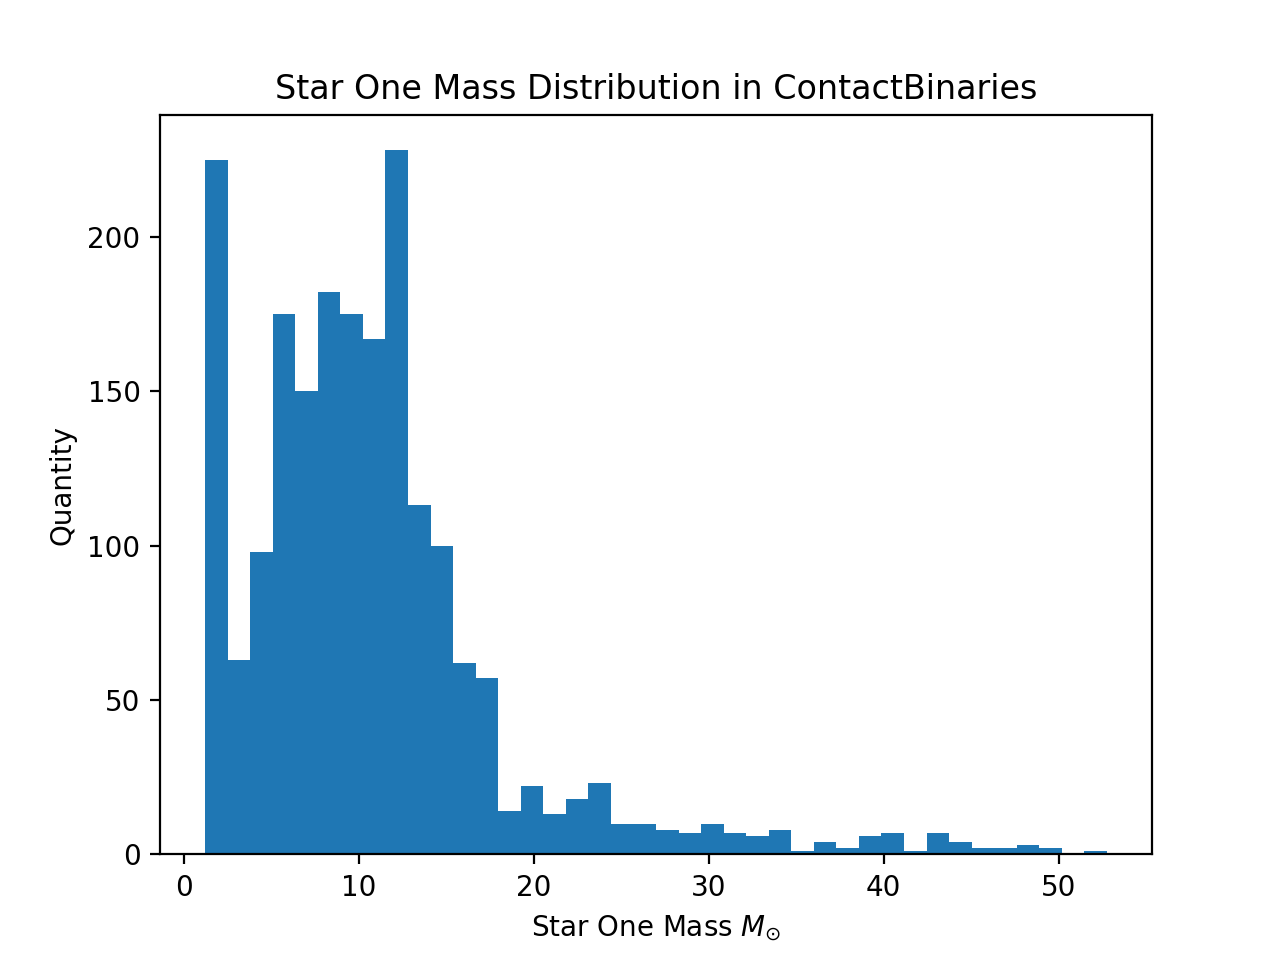
\includegraphics[width=0.22\textwidth]{figs/GeneratedFigs/W_UMa/ContactBinaries_Star_One_Mass_Distribution.png} &
        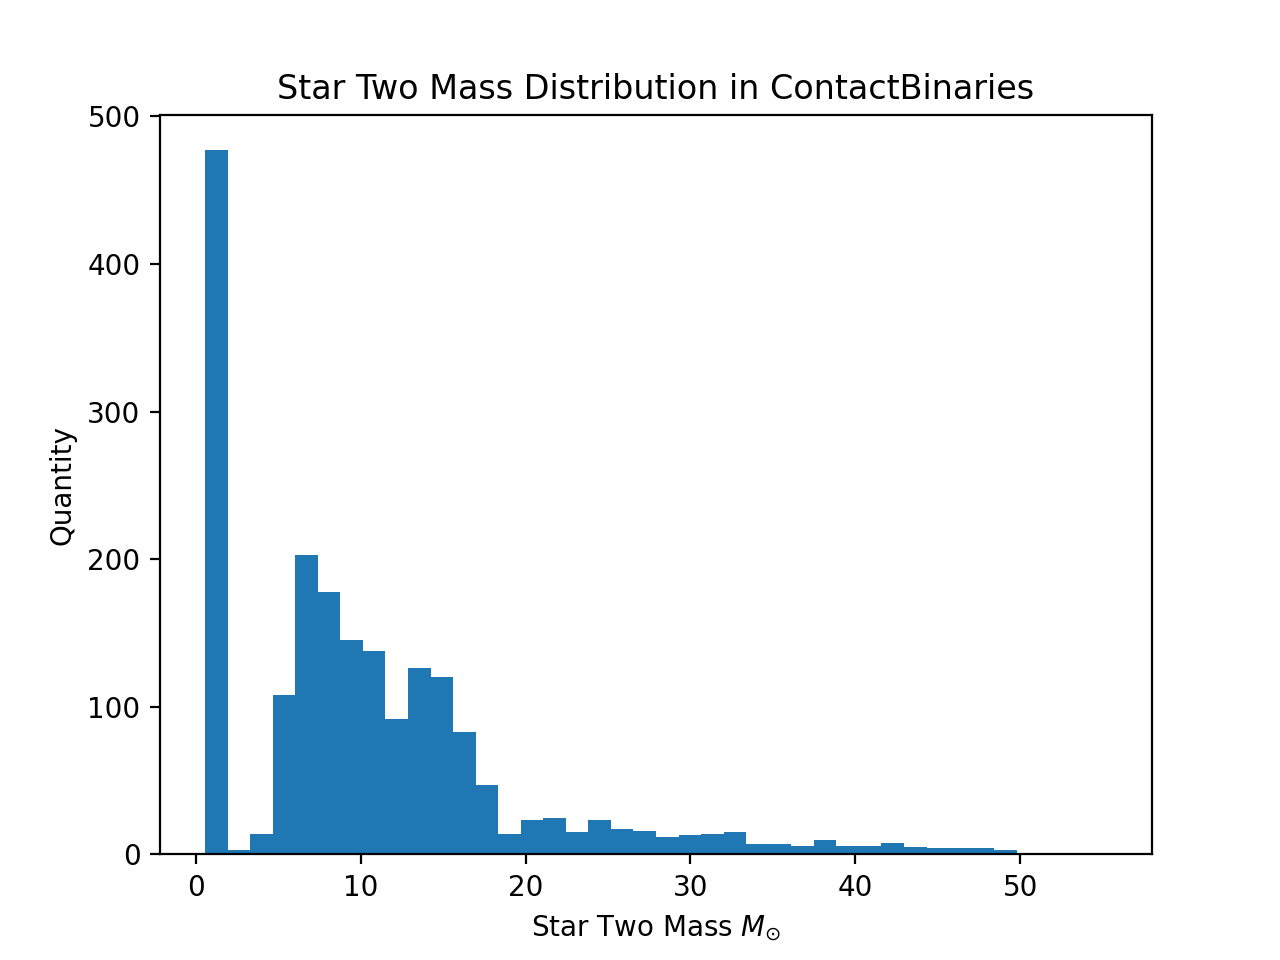
\includegraphics[width=0.22\textwidth]{figs/GeneratedFigs/W_UMa/ContactBinaries_Star_Two_Mass_Distribution.png} &
        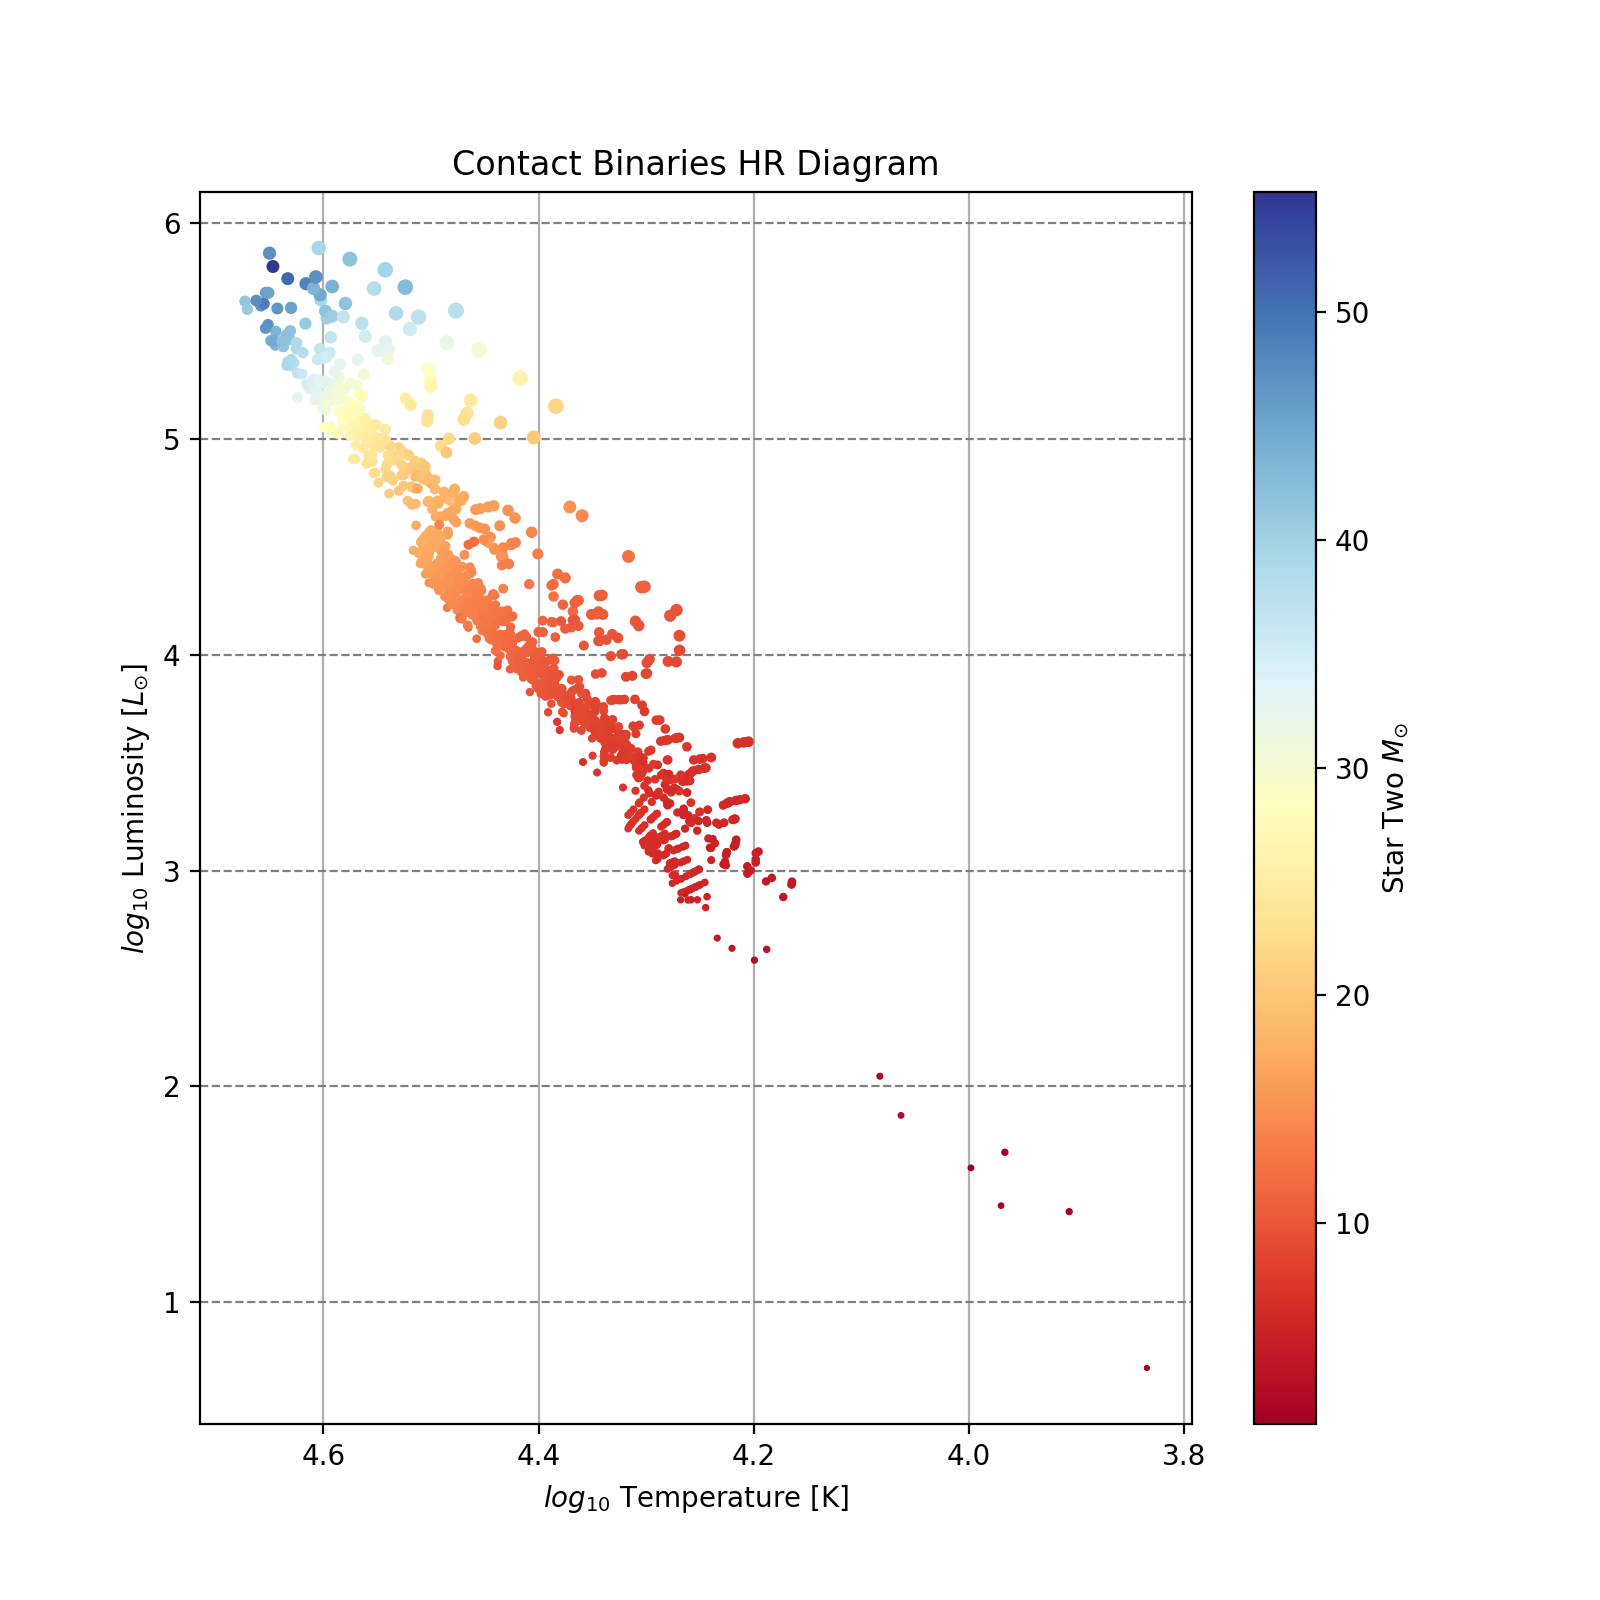
\includegraphics[width=0.22\textwidth]{figs/GeneratedFigs/W_UMa/ContactbinaryHRDiagram.png} &
        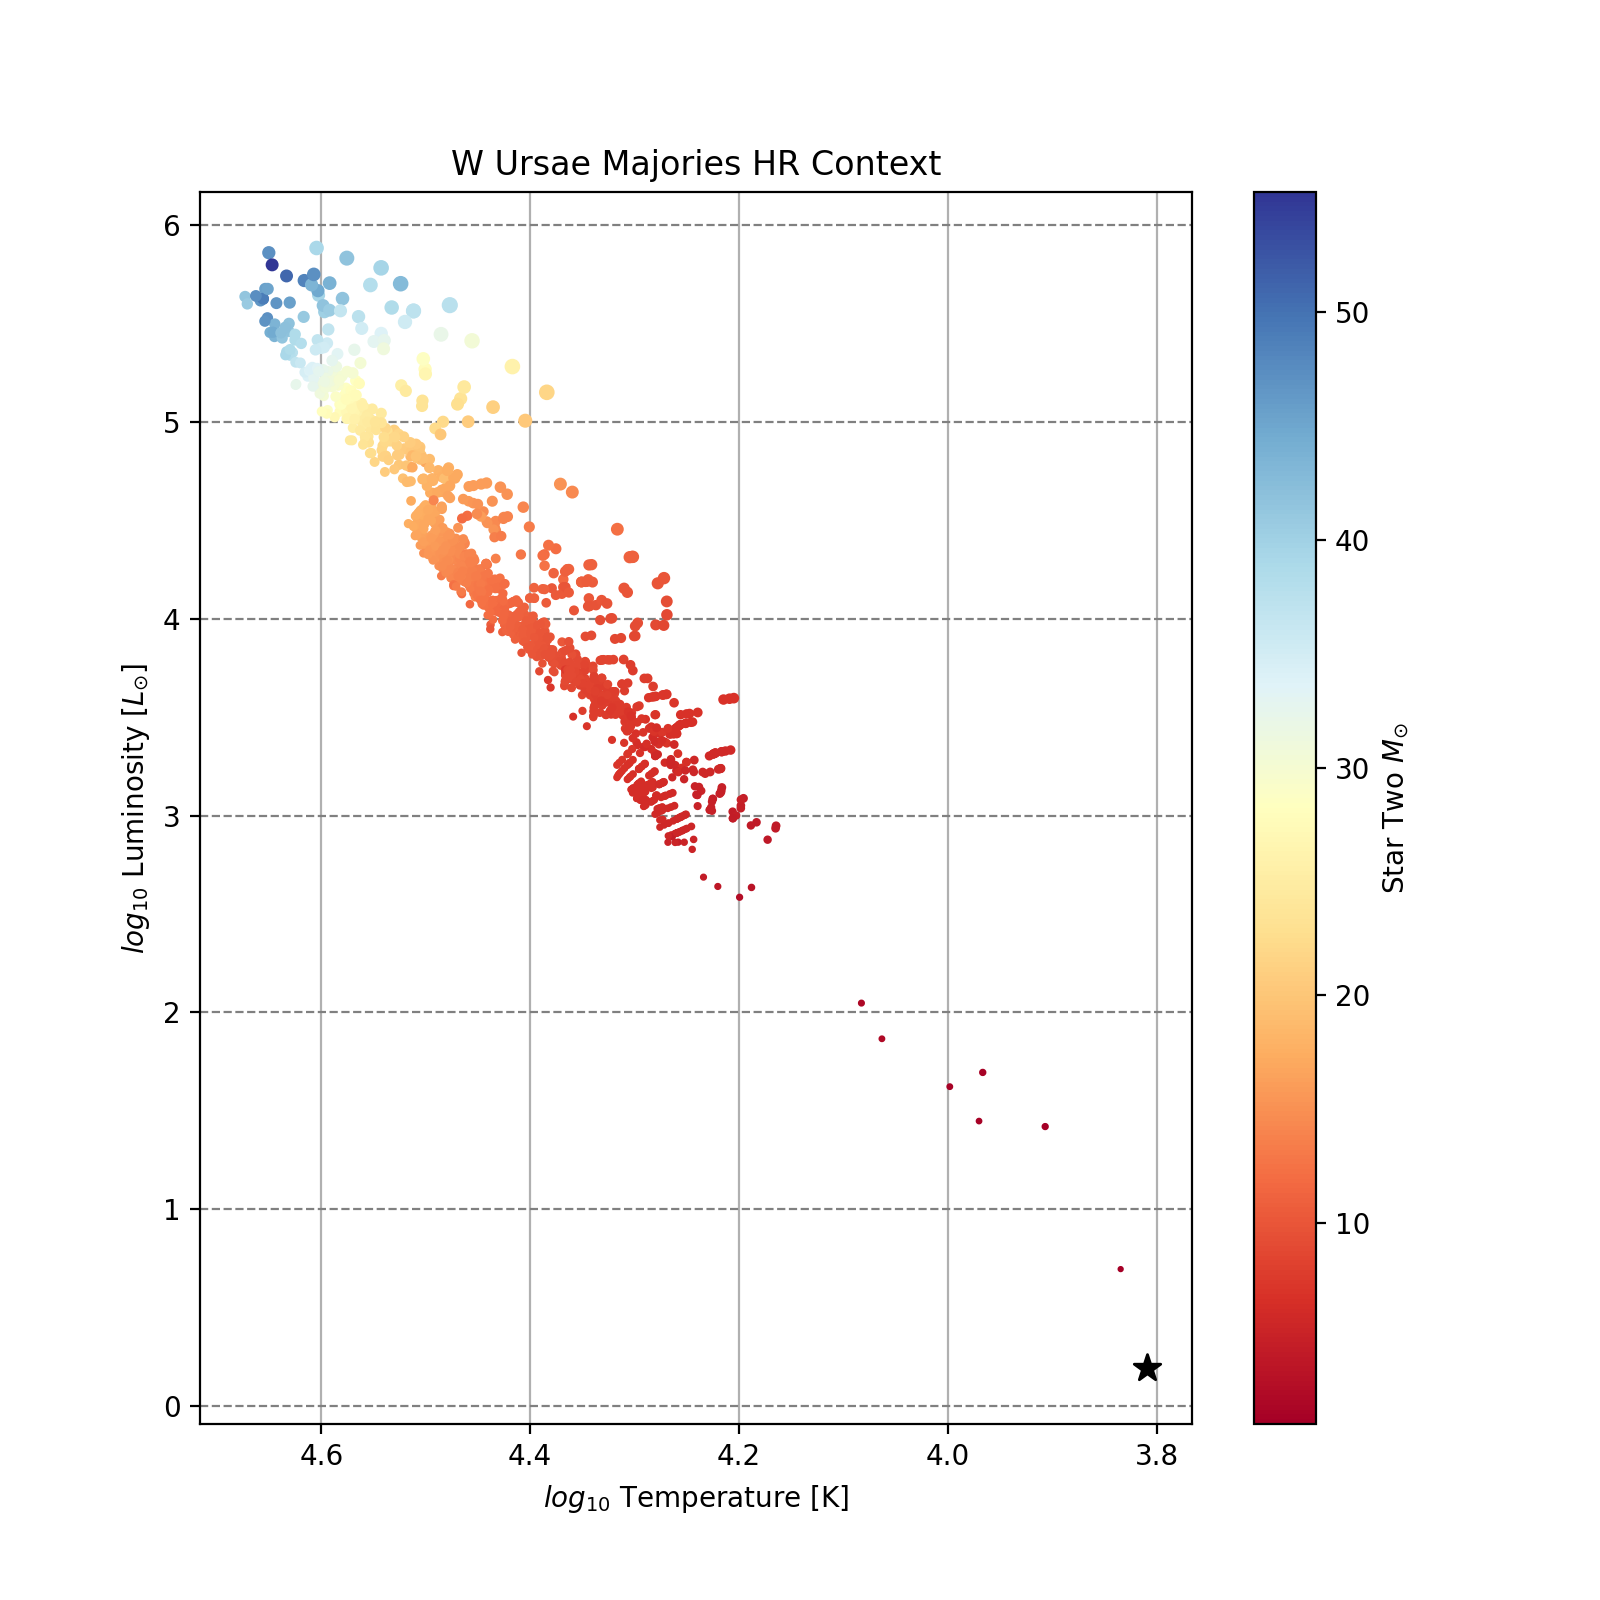
\includegraphics[width=0.22\textwidth]{figs/GeneratedFigs/W_UMa/WUMaHRDiagram.png}\\
        
    \end{tabular}
\end{center}

    
\section{What Would I change}
    % \textit{What would you change about your research process if you were to do it over again?}\\

    If I could redo this I would do it all in the workflow I learned in the process. As I learned \LaTeX~I discovered more and more tools and packages that were suited for my exact needs (section referencing, graph and table labeling, etc.). This meant that as I got further into the paper everything become more streamlined and tidy, but left some of the initial parts crude. If redid this paper I would be able to standardize all of that from the onset, saving me a large amount of time.

    Additionally, I wanted to fully simulate my own grid for one of the stars, however, due to time constraints I was unable to. If I had time to do this again, I would use simulated grids specifically tuned for the systems I was looking at.
\end{document}
